\documentclass[conference]{IEEEtran}
% \IEEEoverridecommandlockouts  % only needed for a \thanks funding footnote; not used here
\usepackage[utf8]{inputenc}
\usepackage[T1]{fontenc}
\usepackage{cite}
\usepackage{amsmath,amssymb,amsfonts}
\usepackage{algorithmic}
\usepackage{graphicx}
\usepackage{textcomp}
\usepackage{xcolor}
\usepackage{booktabs}
\usepackage{array}

\def\BibTeX{{\rm B\kern-.05em{\sc i\kern-.025em b}\kern-.08em
    T\kern-.1667em\lower.7ex\hbox{E}\kern-.125emX}}
\begin{document}

\title{Efficient Transfer Learning for Heritage Building Defect Classification: A Benchmark of Five Convolutional Neural Networks}

\author{
\IEEEauthorblockN{1\textsuperscript{st} Mashrur Rahman}
\IEEEauthorblockA{\textit{Dept. of Computer Science and Engineering}\\
\textit{Ahsanullah University of Science and Technology}\\
Dhaka, Bangladesh\\
mashrur950@gmail.com}
\and
\IEEEauthorblockN{2\textsuperscript{nd} Nahid Asef}
\IEEEauthorblockA{\textit{Dept. of Computer Science and Engineering}\\
\textit{Ahsanullah University of Science and Technology}\\
Dhaka, Bangladesh\\
nahid20asef03@gmail.com}
\and
\IEEEauthorblockN{3\textsuperscript{rd} Nusrat Jahan Oishi}
\IEEEauthorblockA{\textit{Dept. of Computer Science and Engineering}\\
\textit{Ahsanullah University of Science and Technology}\\
Dhaka, Bangladesh\\
oishinusrat359@gmail.com}
\and
\IEEEauthorblockN{4\textsuperscript{th} Chowdhury Ajmayeen Adil}
\IEEEauthorblockA{\textit{Dept. of Computer Science and Engineering}\\
\textit{Ahsanullah University of Science and Technology}\\
Dhaka, Bangladesh\\
ajmayeenadil10@gmail.com}
}

\maketitle

\begin{abstract}
Heritage buildings are irreplaceable cultural assets whose surface defects, if left undetected, accelerate structural deterioration. Manual inspection of these defects is labor intensive, subjective, and often hazardous. This paper presents a systematic transfer-learning benchmark of five convolutional neural network (CNN) architectures---EfficientNet-B0, ResNet-18, EfficientNet-V2-S, DenseNet-121, and MobileNet-V2---for classifying seven surface-defect categories on the publicly available BD3 building-defect dataset (3{,}965 images). Using ImageNet-pretrained backbones, a strong data-augmentation pipeline, and a reproducible training protocol, EfficientNet-B0 attains the highest test accuracy of 93.46\% (95\% Wilson confidence interval $\pm2.0$) and a macro-averaged F1-score of 0.936 with only 4.02M parameters, while all five models exceed 91\% accuracy and a macro-averaged area under the receiver operating characteristic curve of at least 0.993. On the same dataset---which spans both heritage and ordinary facades---our EfficientNet-B0 is on par with the strongest model reported by the original BD3 benchmark under its non-augmented setting (a Vision Transformer, macro-F1 0.932) while using roughly an order of magnitude fewer parameters. We frame this as parameter-efficiency parity rather than a win, because the two studies differ in data split and augmentation protocol and the difference lies within single-run sampling noise. These results indicate that compact, ImageNet-pretrained CNNs offer an accurate and computationally efficient basis for automated building-defect detection that is well suited to resource-constrained edge deployment.
\end{abstract}

\begin{IEEEkeywords}
Heritage building inspection, building defect detection, transfer learning, convolutional neural networks, EfficientNet, image classification, structural health monitoring, edge deployment
\end{IEEEkeywords}

\section{Introduction}
Heritage and historic buildings are irreplaceable cultural assets that deteriorate continuously under environmental exposure to moisture, temperature cycling, biological growth, and mechanical stress. Surface defects such as cracks, algae growth, spalling, staining, and peeling paint are often the earliest visible indicators of underlying structural deterioration. Detecting these defects at an early stage is essential for preventive conservation, efficient allocation of restoration resources, and proper documentation for heritage-preservation authorities~\cite{ref1}. Traditional inspection, however, relies on manual visual surveys that are labor intensive, subjective, difficult to reproduce across inspectors, and frequently hazardous when defects occur at height or on unstable structures.

Recent advances in deep learning and computer vision have enabled the automated analysis of structural defects directly from images, removing the dependence on handcrafted features that characterized earlier image-processing pipelines~\cite{ref5}. In particular, transfer learning with convolutional neural networks (CNNs) pretrained on large-scale datasets such as ImageNet~\cite{ref23} has demonstrated strong performance on image-classification tasks even when the available domain-specific data are limited. By fine-tuning pretrained backbones on defect imagery, high classification accuracy can be obtained from datasets far smaller than those required to train deep networks from scratch~\cite{ref22}.

Despite rapid progress, two practical gaps remain. First, while the recent BD3 benchmark~\cite{ref40} compared several classifiers on this dataset, controlled like-for-like comparisons of \emph{modern, lightweight} CNN backbones under a single transfer-learning recipe are still scarce, and many defect-classification works optimize a single model or report a single accuracy number, making architecture selection difficult for practitioners. Second, much of the literature emphasizes accuracy while overlooking computational efficiency, even though real-world inspection increasingly relies on drones and handheld edge devices where parameter count, memory, and latency are tightly constrained. A model that is marginally more accurate but an order of magnitude larger may be impractical to deploy in the field.

This paper addresses these gaps through a controlled benchmark of five CNN architectures of varying capacity, all fine-tuned under an identical transfer-learning protocol on the BD3 building-defect dataset~\cite{ref40}. The main contributions are as follows:
\begin{itemize}
\item We present a reproducible transfer-learning benchmark of five ImageNet-pretrained CNNs (EfficientNet-B0, ResNet-18, EfficientNet-V2-S, DenseNet-121, and MobileNet-V2) for seven-class building-defect classification, with a fixed random seed, deterministic training, and 95\% confidence intervals on test accuracy.

\item We provide a comprehensive evaluation that goes beyond accuracy, reporting per-class precision, recall, and F1-score, confusion matrices, one-versus-rest ROC/AUC, precision--recall curves with average precision, and an explicit accuracy-versus-parameters efficiency analysis.

\item We position our results against the original BD3 benchmark and show that a compact 4.02M-parameter EfficientNet-B0 reaches a macro-F1 on par with the strongest previously reported model (a Vision Transformer) under BD3's non-augmented setting while using roughly an order of magnitude fewer parameters, providing a strong parameter-efficiency reference for this dataset.

\item We identify EfficientNet-B0 as the most favorable accuracy--efficiency trade-off among the evaluated models, making it a practical candidate for edge-deployed heritage-inspection systems.
\end{itemize}
\section{Related Work}

The visual inspection of building facades and civil infrastructure has shifted decisively from manual surveys and handcrafted-feature pipelines toward data-driven deep learning, a transition documented in several recent reviews \cite{ref1,ref2,ref3,ref4}. Spencer~\textit{et al.} survey the broad landscape of computer-vision-based inspection and monitoring, including damage characterization and aerial imaging \cite{ref2}, while Sony~\textit{et al.} provide a systematic taxonomy of convolutional neural network (CNN)-based structural condition assessment \cite{ref3}, and Ameri~\textit{et al.} organize industrial surface-defect methods into classification, detection, and segmentation families across supervised and unsupervised regimes \cite{ref4}. Within the cultural-heritage niche specifically, Mishra and Lourenço review the state of artificial-intelligence-assisted visual inspection and identify persistent gaps in benchmarking and dataset availability \cite{ref1}. These surveys collectively frame the problem space that the present work addresses through a systematic multi-architecture classification benchmark.

Early CNN approaches established the feasibility of learning defect representations directly from images rather than engineering features by hand. Cha~\textit{et al.} demonstrated that a CNN could detect concrete cracks robustly under varying lighting and texture, outperforming traditional edge- and threshold-based techniques \cite{ref5}, and the release of annotated benchmarks such as SDNET2018 \cite{ref6} catalyzed reproducible study of non-contact crack detection. Subsequent work extended this paradigm from binary crack recognition to broader building-defect classification: Shomal~Zadeh~\textit{et al.} fine-tuned ImageNet-pretrained backbones including ResNet and EfficientNet variants for concrete-crack classification \cite{ref7}, Siva~Rama~Krishnan~\textit{et al.} compared multiple deep models for crack detection in buildings \cite{ref8}, and Perez~\textit{et al.} classified defects such as mold, deterioration, and stain using a pretrained VGG-16 compared against ResNet-50 and Inception \cite{ref9}. For facade defects specifically, Guo~\textit{et al.} introduced a meta-learning CNN that mitigates class imbalance under a layer-based defect taxonomy \cite{ref10}, while Mundt~\textit{et al.} released the CODEBRIM benchmark for multi-target concrete-defect classification spanning cracks, spallation, efflorescence, exposed bars, and corrosion \cite{ref11}. These studies motivate our per-image, multi-class formulation but typically evaluate a narrow set of architectures.

Where defects must be located rather than merely recognized, the literature turns to object detection. Cha~\textit{et al.} employed a region-based (Faster R-CNN) detector for quasi-real-time simultaneous detection of multiple damage types \cite{ref12}, Lee~\textit{et al.} adapted Faster R-CNN to multi-class facade-defect detection in their MultiDefectNet \cite{ref13}, and recent real-time detectors based on the YOLO family push toward joint detection and segmentation of cracks \cite{ref14}. For pixel-level localization, semantic and instance segmentation architectures form a distinct lineage: fully convolutional networks established end-to-end dense prediction \cite{ref15}, the U-Net encoder-decoder with skip connections \cite{ref16} and its nested UNet++ refinement \cite{ref17} became the backbone of most crack-localization systems, and Mask R-CNN \cite{ref18} extended detection to per-instance masks. Domain-specific segmentation models such as DeepCrack \cite{ref19} and U-Net-based pavement crack segmentation \cite{ref20}, together with consolidated benchmarks like CrackSeg9k that compare U-Net, DeepLabV3+, Swin-UNet, and Mask R-CNN \cite{ref21}, illustrate both the maturity and the annotation cost of this paradigm. We treat segmentation as a natural extension of, rather than a replacement for, the classification task benchmarked here.

A recurring obstacle across these tasks is the scarcity of labeled defect imagery, which transfer learning directly addresses. Gao and Mosalam introduced the ``Structural ImageNet'' paradigm, transferring features from ImageNet-pretrained VGG-16 \cite{ref23} to overcome small-dataset limitations in structural damage recognition \cite{ref22}. This fine-tuning strategy underpins our methodology and is realized through five backbone families: ResNet \cite{ref24}, DenseNet \cite{ref25}, MobileNet-V2 \cite{ref26}, EfficientNet \cite{ref27}, and EfficientNet-V2 \cite{ref28}, each evaluated under ImageNet initialization. Closest to our setting, Dais~\textit{et al.} benchmarked transfer-learning CNNs for crack classification and segmentation on masonry surfaces \cite{ref29}, directly paralleling the facade-defect focus of this study.

The heritage-building context introduces additional material diversity and conservation constraints that have spurred a dedicated body of work. Samhouri~\textit{et al.} classified heritage-facade damage such as erosion, material loss, and stone color change with a CNN reaching roughly 95\% accuracy \cite{ref30}; Hacıefendioğlu~\textit{et al.} \cite{ref31} and Huang~\textit{et al.} \cite{ref34} targeted crack detection on historical masonry and cultural-heritage surfaces; Fu and Angkawisittpan addressed heritage-facade surface defects more broadly \cite{ref32}; Karimi~\textit{et al.} applied a YOLO detector across stone, brick, and concrete heritage materials \cite{ref33}; and Chen~\textit{et al.} built a pipeline for surface-pathology detection on historic masonry buildings spanning cracks, spalling, and biological growth \cite{ref35}. In parallel, UAV-based acquisition has become a practical front end for these systems, feeding deep classifiers and detectors with drone-captured imagery \cite{ref36,ref37,ref38}, and large new datasets continue to expand the scale and diversity of building-surface defect imagery \cite{ref39}. Most directly relevant to this study, the BD3 benchmark of Kottari and Arjunan~\cite{ref40} released the seven-class building-defect dataset used here and evaluated five classifiers (a Vision Transformer, AlexNet, VGG-16, ResNet-18, and MobileNet-V2) on it. The present work complements~\cite{ref40} by fine-tuning a different, efficiency-oriented set of modern CNN backbones under a single augmentation and training recipe, and by analyzing the accuracy--parameter trade-off explicitly; Section~\ref{sec:comparison} positions our results against that benchmark in detail.

\section{Dataset Description}
The experiments in this study use the BD3 (Building Defects Detection) dataset~\cite{ref40}, a publicly available benchmark obtained from the Kaggle repository. The dataset contains 3{,}965 RGB images of surface conditions commonly observed on building facades, organized into seven classes: \textit{algae}, \textit{major crack}, \textit{minor crack}, \textit{peeling}, \textit{plain} (no defect), \textit{spalling}, and \textit{stain}. These categories span both heritage and ordinary facades and represent the typical structural and surface-level deterioration relevant to heritage preservation; we therefore treat the present results as evidence that the approach is \emph{applicable} to heritage inspection rather than as a heritage-only validation.

As summarized in Table~\ref{tab:dataset}, the dataset is relatively well balanced, with the number of images per class ranging from 500 (\textit{spalling}) to 624 (\textit{minor crack}). This balanced distribution reduces the impact of class imbalance during training and evaluation. Fig.~\ref{fig:split_dist} shows that the balance is preserved across the training, validation, and test partitions.

\begin{table}[htbp]
\caption{Class Distribution of the BD3 Dataset}
\label{tab:dataset}
\centering
\begin{tabular}{lc}
\toprule
\textbf{Defect Class} & \textbf{Number of Images} \\
\midrule
algae        & 620 \\
major\_crack & 580 \\
minor\_crack & 624 \\
peeling      & 520 \\
plain        & 600 \\
spalling     & 500 \\
stain        & 521 \\
\midrule
\textbf{Total} & \textbf{3{,}965} \\
\bottomrule
\end{tabular}
\end{table}

\begin{figure}[htbp]
\centerline{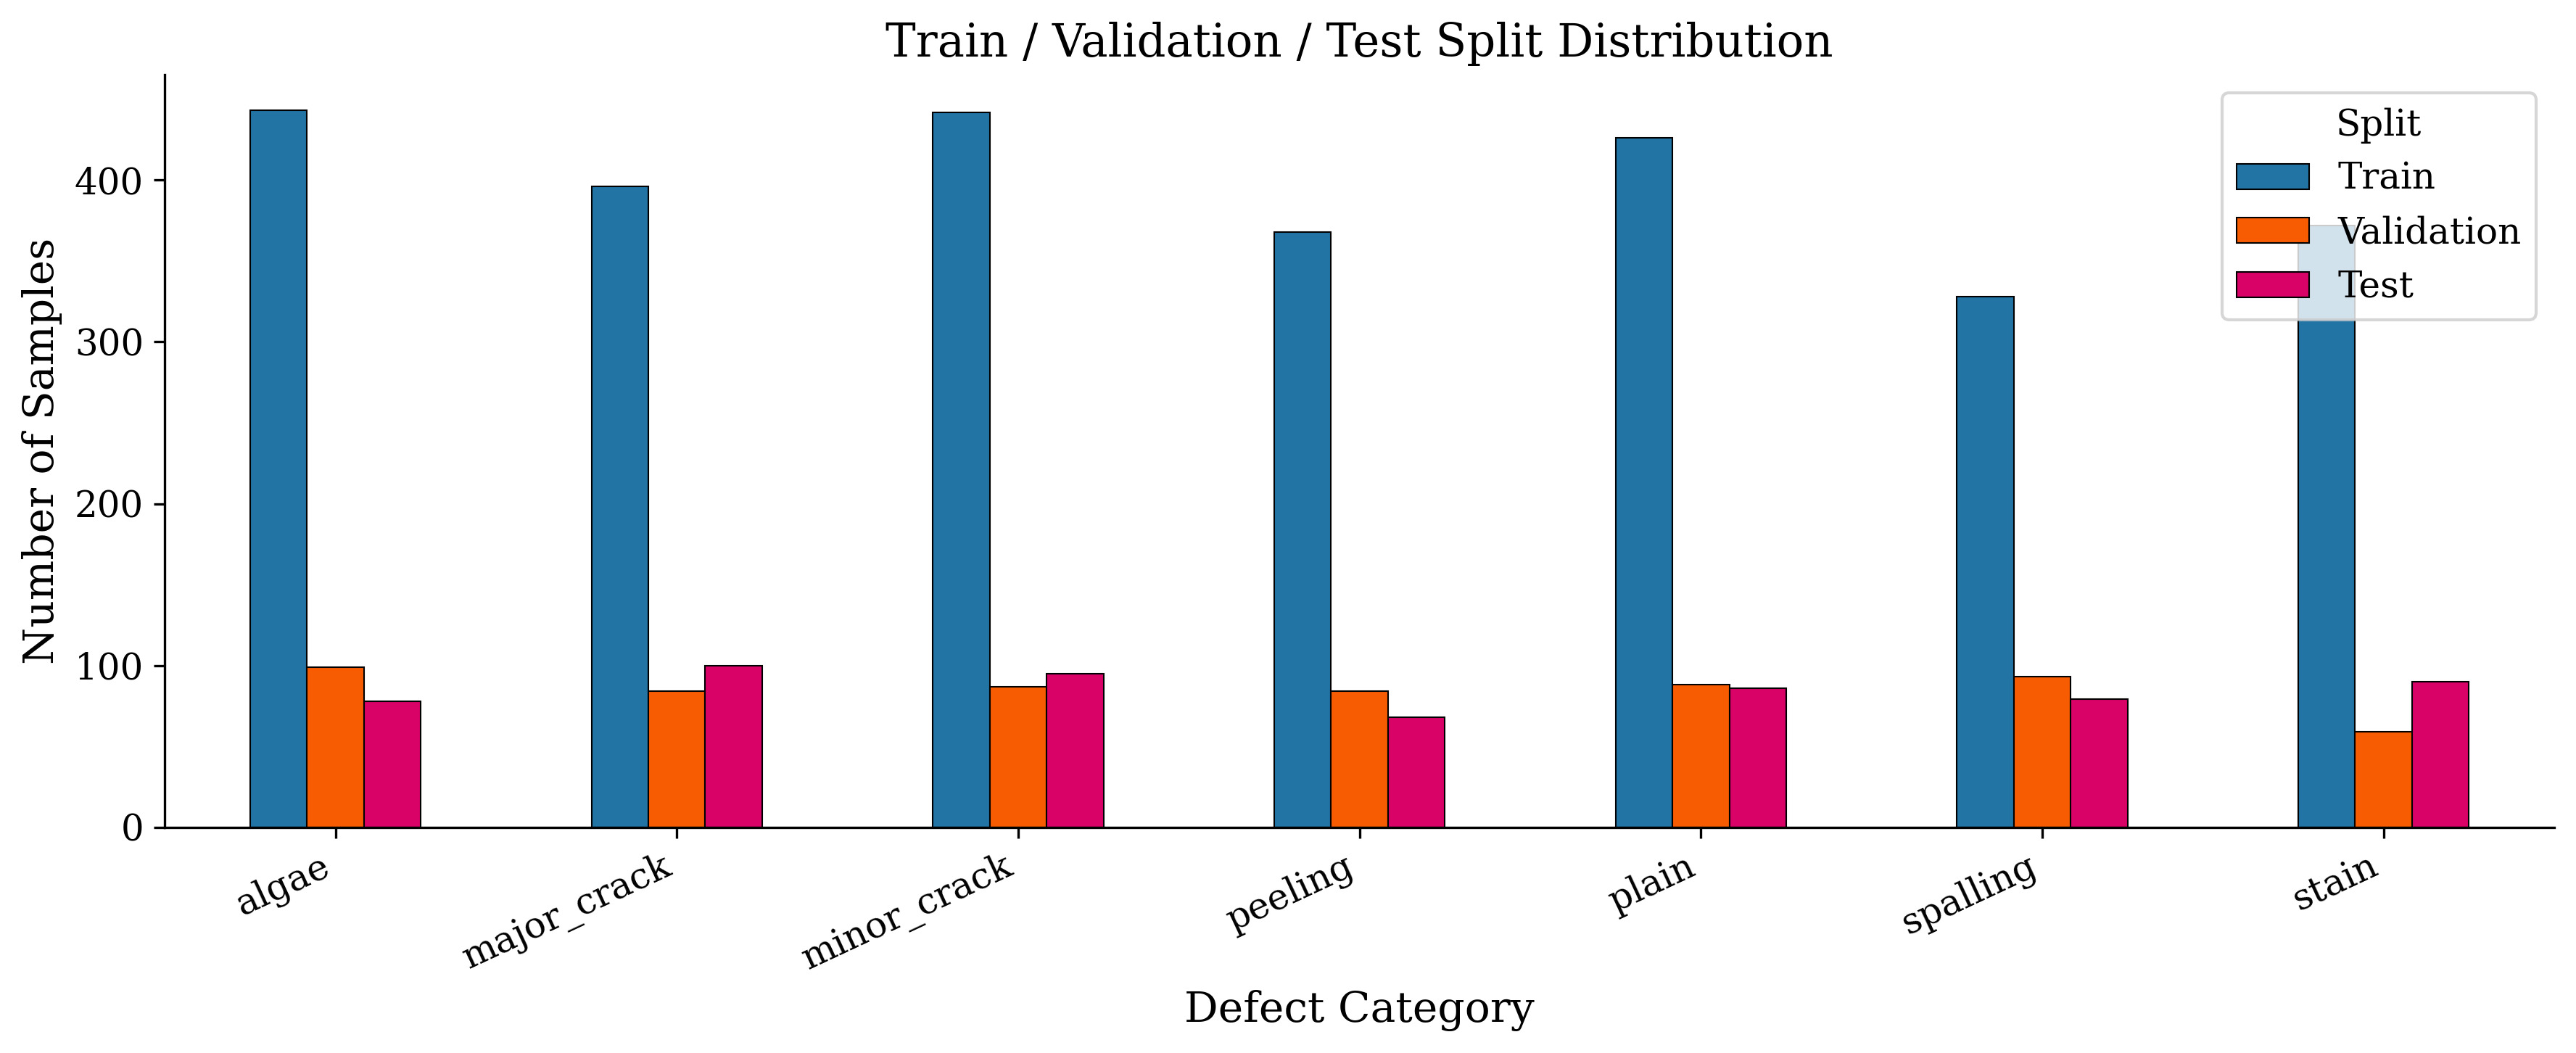
\includegraphics[width=\linewidth]{fig_split_distribution.jpg}}
\caption{Per-class image counts across the training, validation, and test splits of the BD3 dataset.}
\label{fig:split_dist}
\end{figure}

All images were resized to a fixed resolution of $224\times224$ pixels to maintain compatibility with the CNN architectures evaluated. For model development, the dataset was partitioned by a non-stratified random shuffle under a fixed seed (42) into 70\% training, 15\% validation, and 15\% testing subsets, yielding 2{,}775 training, 594 validation, and 596 testing images. Because the dataset is approximately balanced, random shuffling preserves the class distribution across splits reasonably well, although it does not guarantee identical per-class proportions. To avoid optimistic evaluation, a custom dataset wrapper applied data-augmentation transforms only to the training subset, while validation and test samples received identical, augmentation-free preprocessing. Because the split is image-level rather than building-level, near-duplicate views of the same surface could in principle fall into different subsets; we note this as a limitation in Section~\ref{sec:limitations}.

\section{Methodology}
The proposed system follows a four-stage deep-learning pipeline for automated classification of building surface defects: data preprocessing and augmentation, model-architecture selection, training strategy, and performance evaluation.

\textbf{Data Preprocessing and Augmentation.}
To ensure a consistent input size, all images were resized to $224\times224$ pixels. Data augmentation was applied to the training subset only, to improve generalization and reduce overfitting. The augmentation pipeline comprised random horizontal and vertical flipping, random rotation up to $\pm15^{\circ}$, color jittering (brightness, contrast, and saturation $0.3$; hue $0.2$), random affine transformations with translation up to $10\%$ and scaling between $0.9$ and $1.1$, and random erasing with probability $0.3$. These transformations simulate the variations in lighting, orientation, and partial occlusion encountered in real-world inspection imagery. All images were converted to tensors and normalized using the standard ImageNet mean and standard deviation to match the statistics expected by the pretrained backbones. Validation and test images received only resizing and normalization.

\textbf{Model Architectures.}
Five CNN architectures were evaluated: EfficientNet-B0~\cite{ref27}, ResNet-18~\cite{ref24}, EfficientNet-V2-S~\cite{ref28}, DenseNet-121~\cite{ref25}, and MobileNet-V2~\cite{ref26}. Each model was initialized with ImageNet-pretrained weights~\cite{ref23} and fine-tuned for the defect-classification task. The final classifier of each network was replaced with a dropout layer (probability $0.3$) followed by a fully connected layer producing seven output logits corresponding to the defect categories. All backbone layers were left trainable (full fine-tuning); no layers were frozen and no warmup or two-stage schedule was used.

\textbf{Training Strategy.}
All models were trained under an identical supervised protocol using the Adam optimizer with an initial learning rate of $5\times10^{-4}$ and weight decay of $1\times10^{-4}$, a batch size of 32, and the cross-entropy loss. A \texttt{ReduceLROnPlateau} scheduler halved the learning rate (factor $0.5$) after three epochs without improvement in validation loss. Training ran for a maximum of 30 epochs, and early stopping with a patience of seven epochs monitored validation accuracy, retaining the weights of the best-performing epoch. To ensure reproducibility, a single global random seed (42) was fixed across Python, NumPy, and PyTorch---governing the data split, classifier-head initialization, and augmentation sampling---and deterministic cuDNN behavior was enabled.

\textbf{Evaluation Framework.}
Model performance was assessed on the held-out test set using multiple complementary metrics. Overall performance was measured by test accuracy, and class-level performance by precision, recall, and F1-score (reported both per class and as macro and weighted averages). Because the test set comprises a single held-out partition of 596 images, we additionally report 95\% Wilson score confidence intervals for test accuracy. Confusion matrices, in both absolute and row-normalized form, were generated to visualize inter-class errors. Receiver operating characteristic (ROC) curves and the corresponding area under the curve (AUC) were computed using a one-versus-rest scheme, together with precision--recall curves and average precision (AP). Finally, model efficiency was analyzed by relating test accuracy to parameter count, to identify architectures that balance accuracy and computational cost.

\textbf{Implementation Details.}
All experiments were implemented in PyTorch and torchvision using the \texttt{IMAGENET1K\_V1} pretrained weight enumerations, and run under Python~3.12 on a single NVIDIA GPU via Google Colaboratory. Reported parameter counts are totals (backbone plus classifier head). The determinism described above holds for the stated software and hardware configuration; exact numerical reproduction on different CUDA/cuDNN versions or GPU models may vary slightly.

\section{Experimental Results}

\subsection{Overall Model Comparison}
All five models were trained and evaluated under the identical protocol described above. Table~\ref{tab:model_comparison} reports the parameter count, best validation accuracy, test accuracy (with its 95\% Wilson confidence interval), and macro-averaged F1-score for each architecture, sorted by test accuracy. EfficientNet-B0 achieved the highest test accuracy of 93.46\% with only 4.02M parameters, and all five architectures exceeded 91\% test accuracy, confirming that ImageNet transfer learning is highly effective for this task. Because evaluation uses a single held-out test set of 596 images, the 95\% confidence intervals (each approximately $\pm2$ points) overlap across all five models; the differences should therefore be read as a consistent high-accuracy band rather than a statistically separable ranking. The accuracy--efficiency relationship is visualized in Fig.~\ref{fig:eff}: EfficientNet-B0 occupies the most favorable region (high accuracy, low parameter count), whereas EfficientNet-V2-S---the largest model at 20.19M parameters---did not achieve higher accuracy, suggesting that additional capacity was not advantageous under the present data scale and training budget.

\begin{table}[htbp]
\caption{Model Comparison on the Test Set. Test accuracy is shown with its 95\% Wilson confidence interval ($n=596$); the intervals overlap across all models.}
\label{tab:model_comparison}
\centering
\begin{tabular}{lcccc}
\toprule
\textbf{Model} & \textbf{Params} & \textbf{Val Acc} & \textbf{Test Acc} & \textbf{Macro} \\
 & \textbf{(M)} & \textbf{(\%)} & \textbf{(\%)} & \textbf{F1} \\
\midrule
EfficientNet-B0   & 4.02  & 94.61 & \textbf{93.46\,$\pm$2.0} & \textbf{0.936} \\
ResNet-18         & 11.18 & 93.10 & 92.62\,$\pm$2.1 & 0.927 \\
MobileNet-V2      & 2.23  & 93.94 & 91.78\,$\pm$2.2 & 0.918 \\
DenseNet-121      & 6.96  & 91.41 & 91.61\,$\pm$2.2 & 0.918 \\
EfficientNet-V2-S & 20.19 & 93.43 & 91.44\,$\pm$2.3 & 0.915 \\
\bottomrule
\end{tabular}
\end{table}

\begin{figure}[htbp]
\centerline{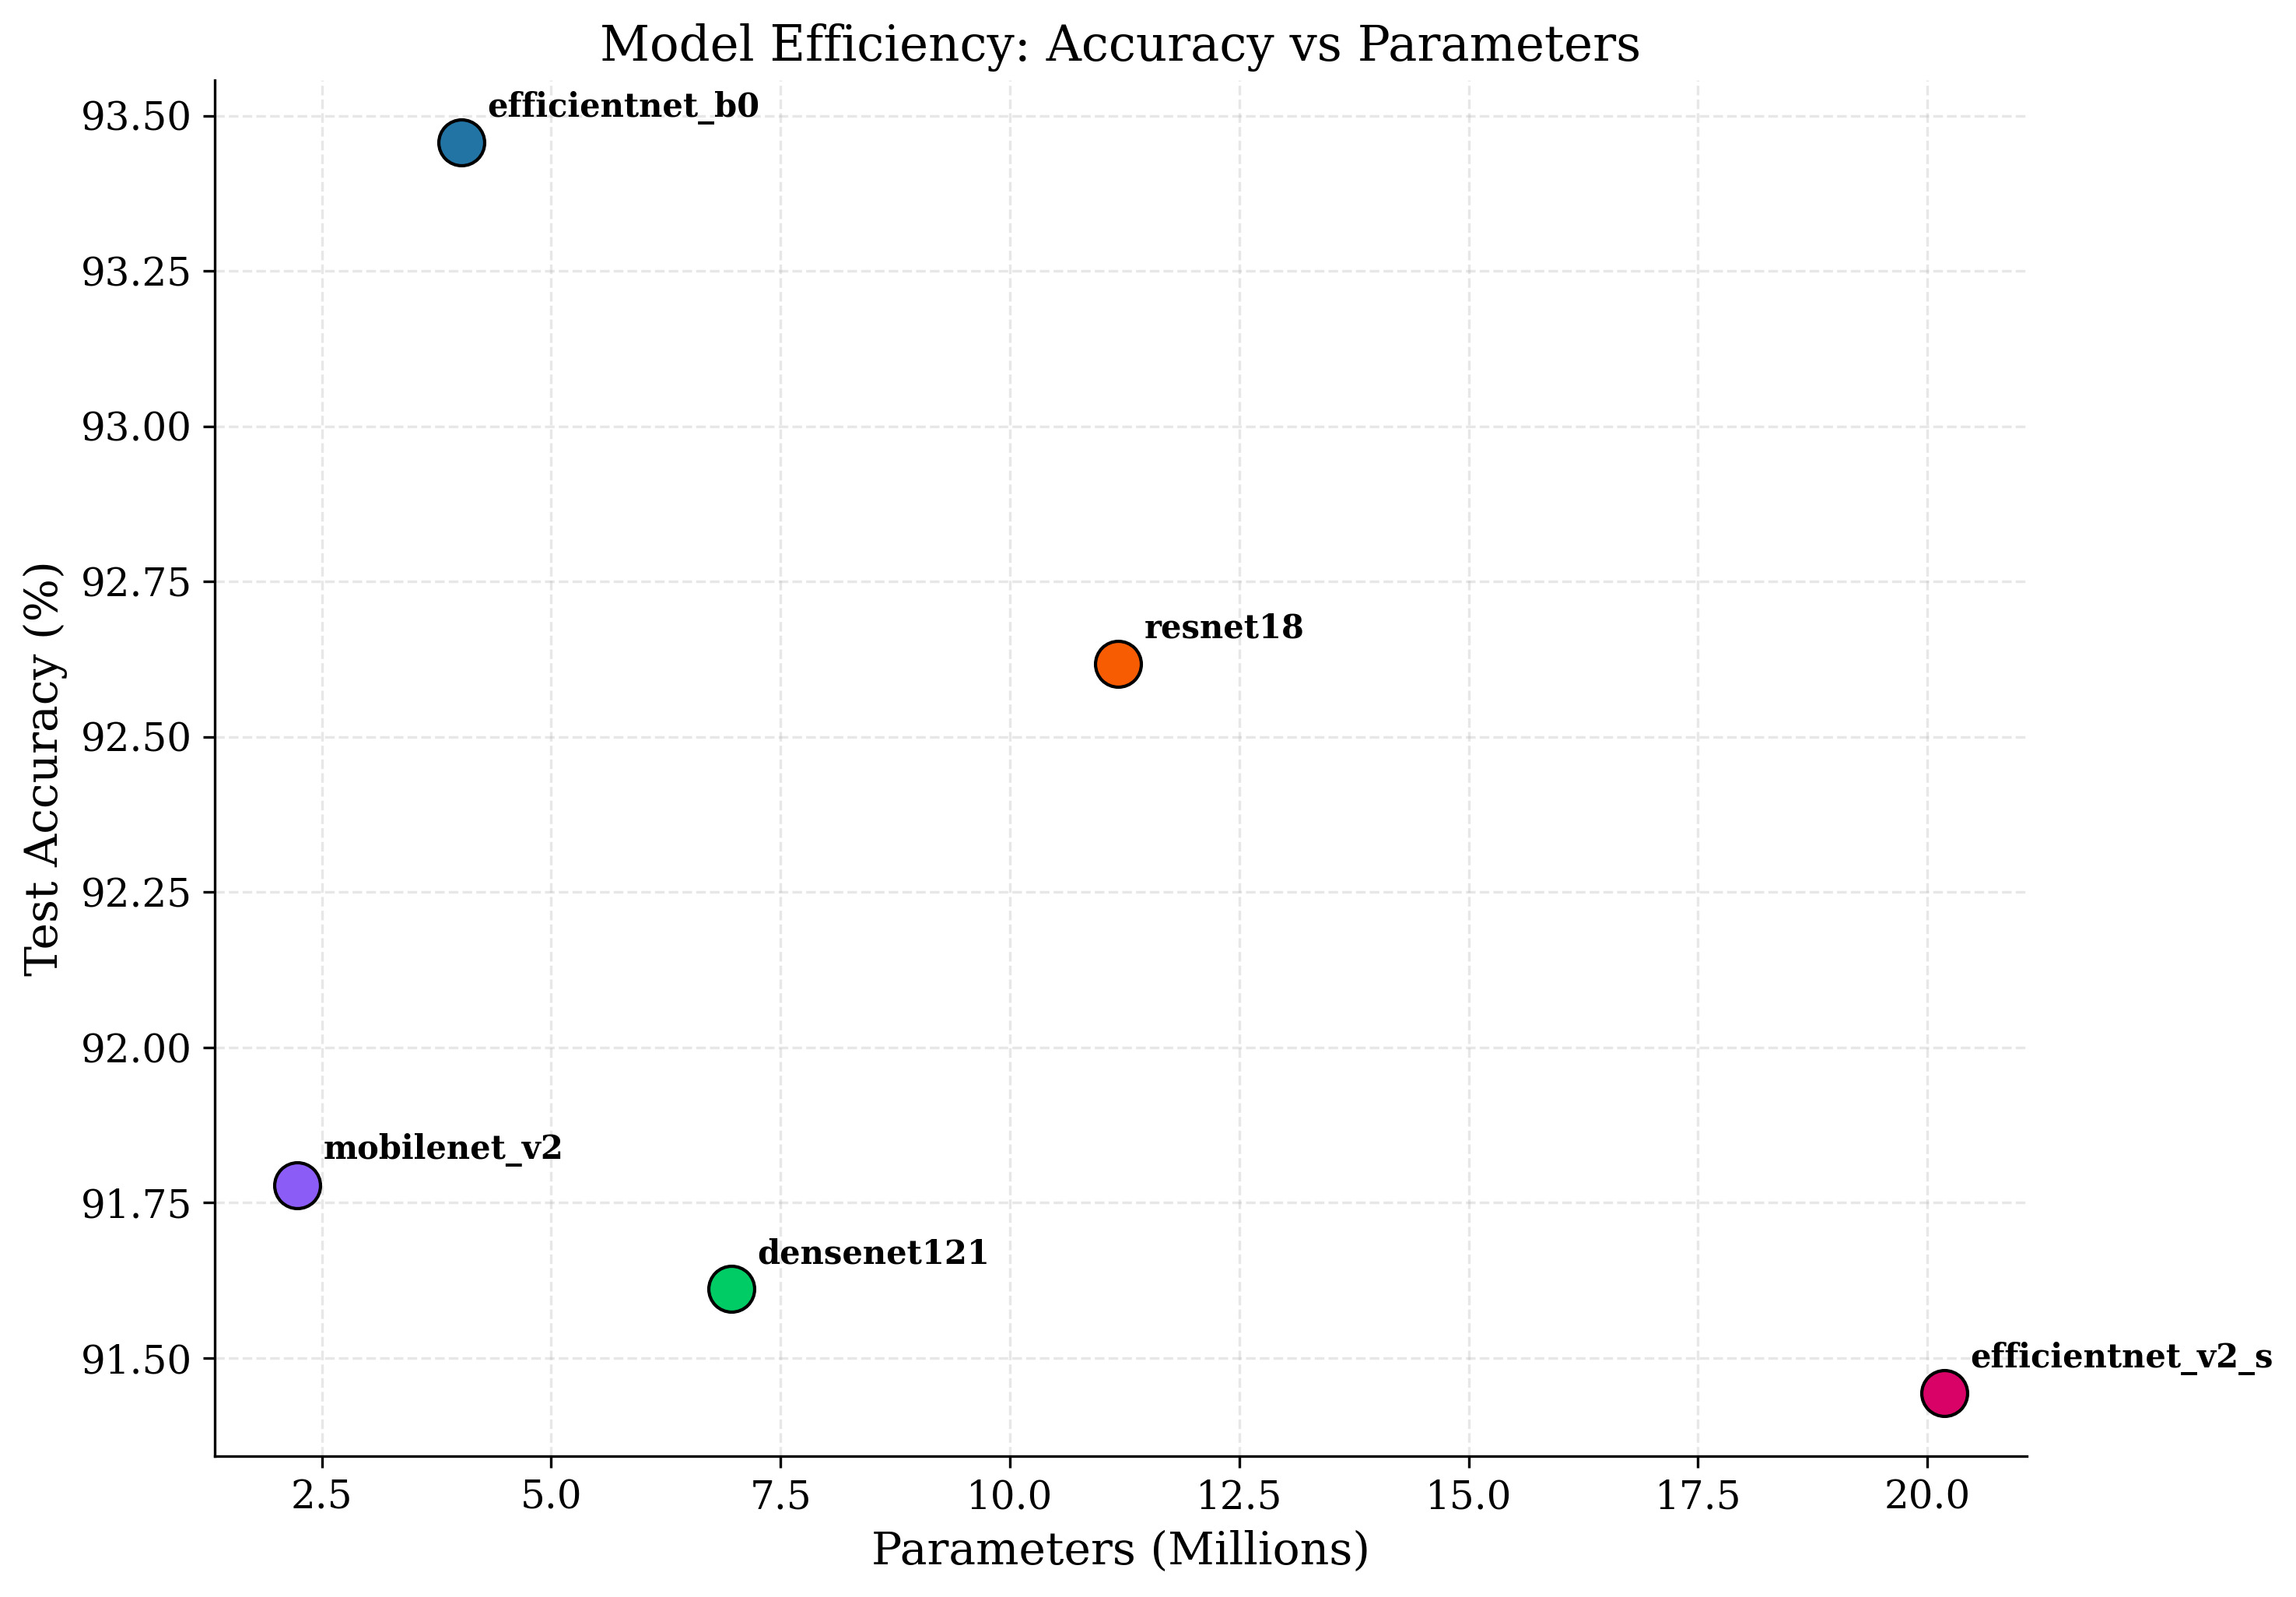
\includegraphics[width=\linewidth]{fig_accuracy_vs_params.jpg}}
\caption{Test accuracy versus parameter count on the BD3 test set. EfficientNet-B0 offers the best accuracy--efficiency trade-off; the largest model, EfficientNet-V2-S, is not the most accurate.}
\label{fig:eff}
\end{figure}

\subsection{Training Dynamics}
All architectures converged rapidly under transfer learning. EfficientNet-B0 reached 86.87\% validation accuracy within the first epoch and its best validation accuracy of 94.61\% by epoch~16, after which early stopping halted training. Fig.~\ref{fig:acc_curves} shows the training and validation accuracy trajectories for all five models on the BD3 dataset. The generalization gap between training and validation accuracy remained small (below roughly 3--5\% at convergence) for all models, indicating that the augmentation and regularization strategy effectively limited overfitting; this behavior is examined further in the Discussion.

\begin{figure*}[t]
\centerline{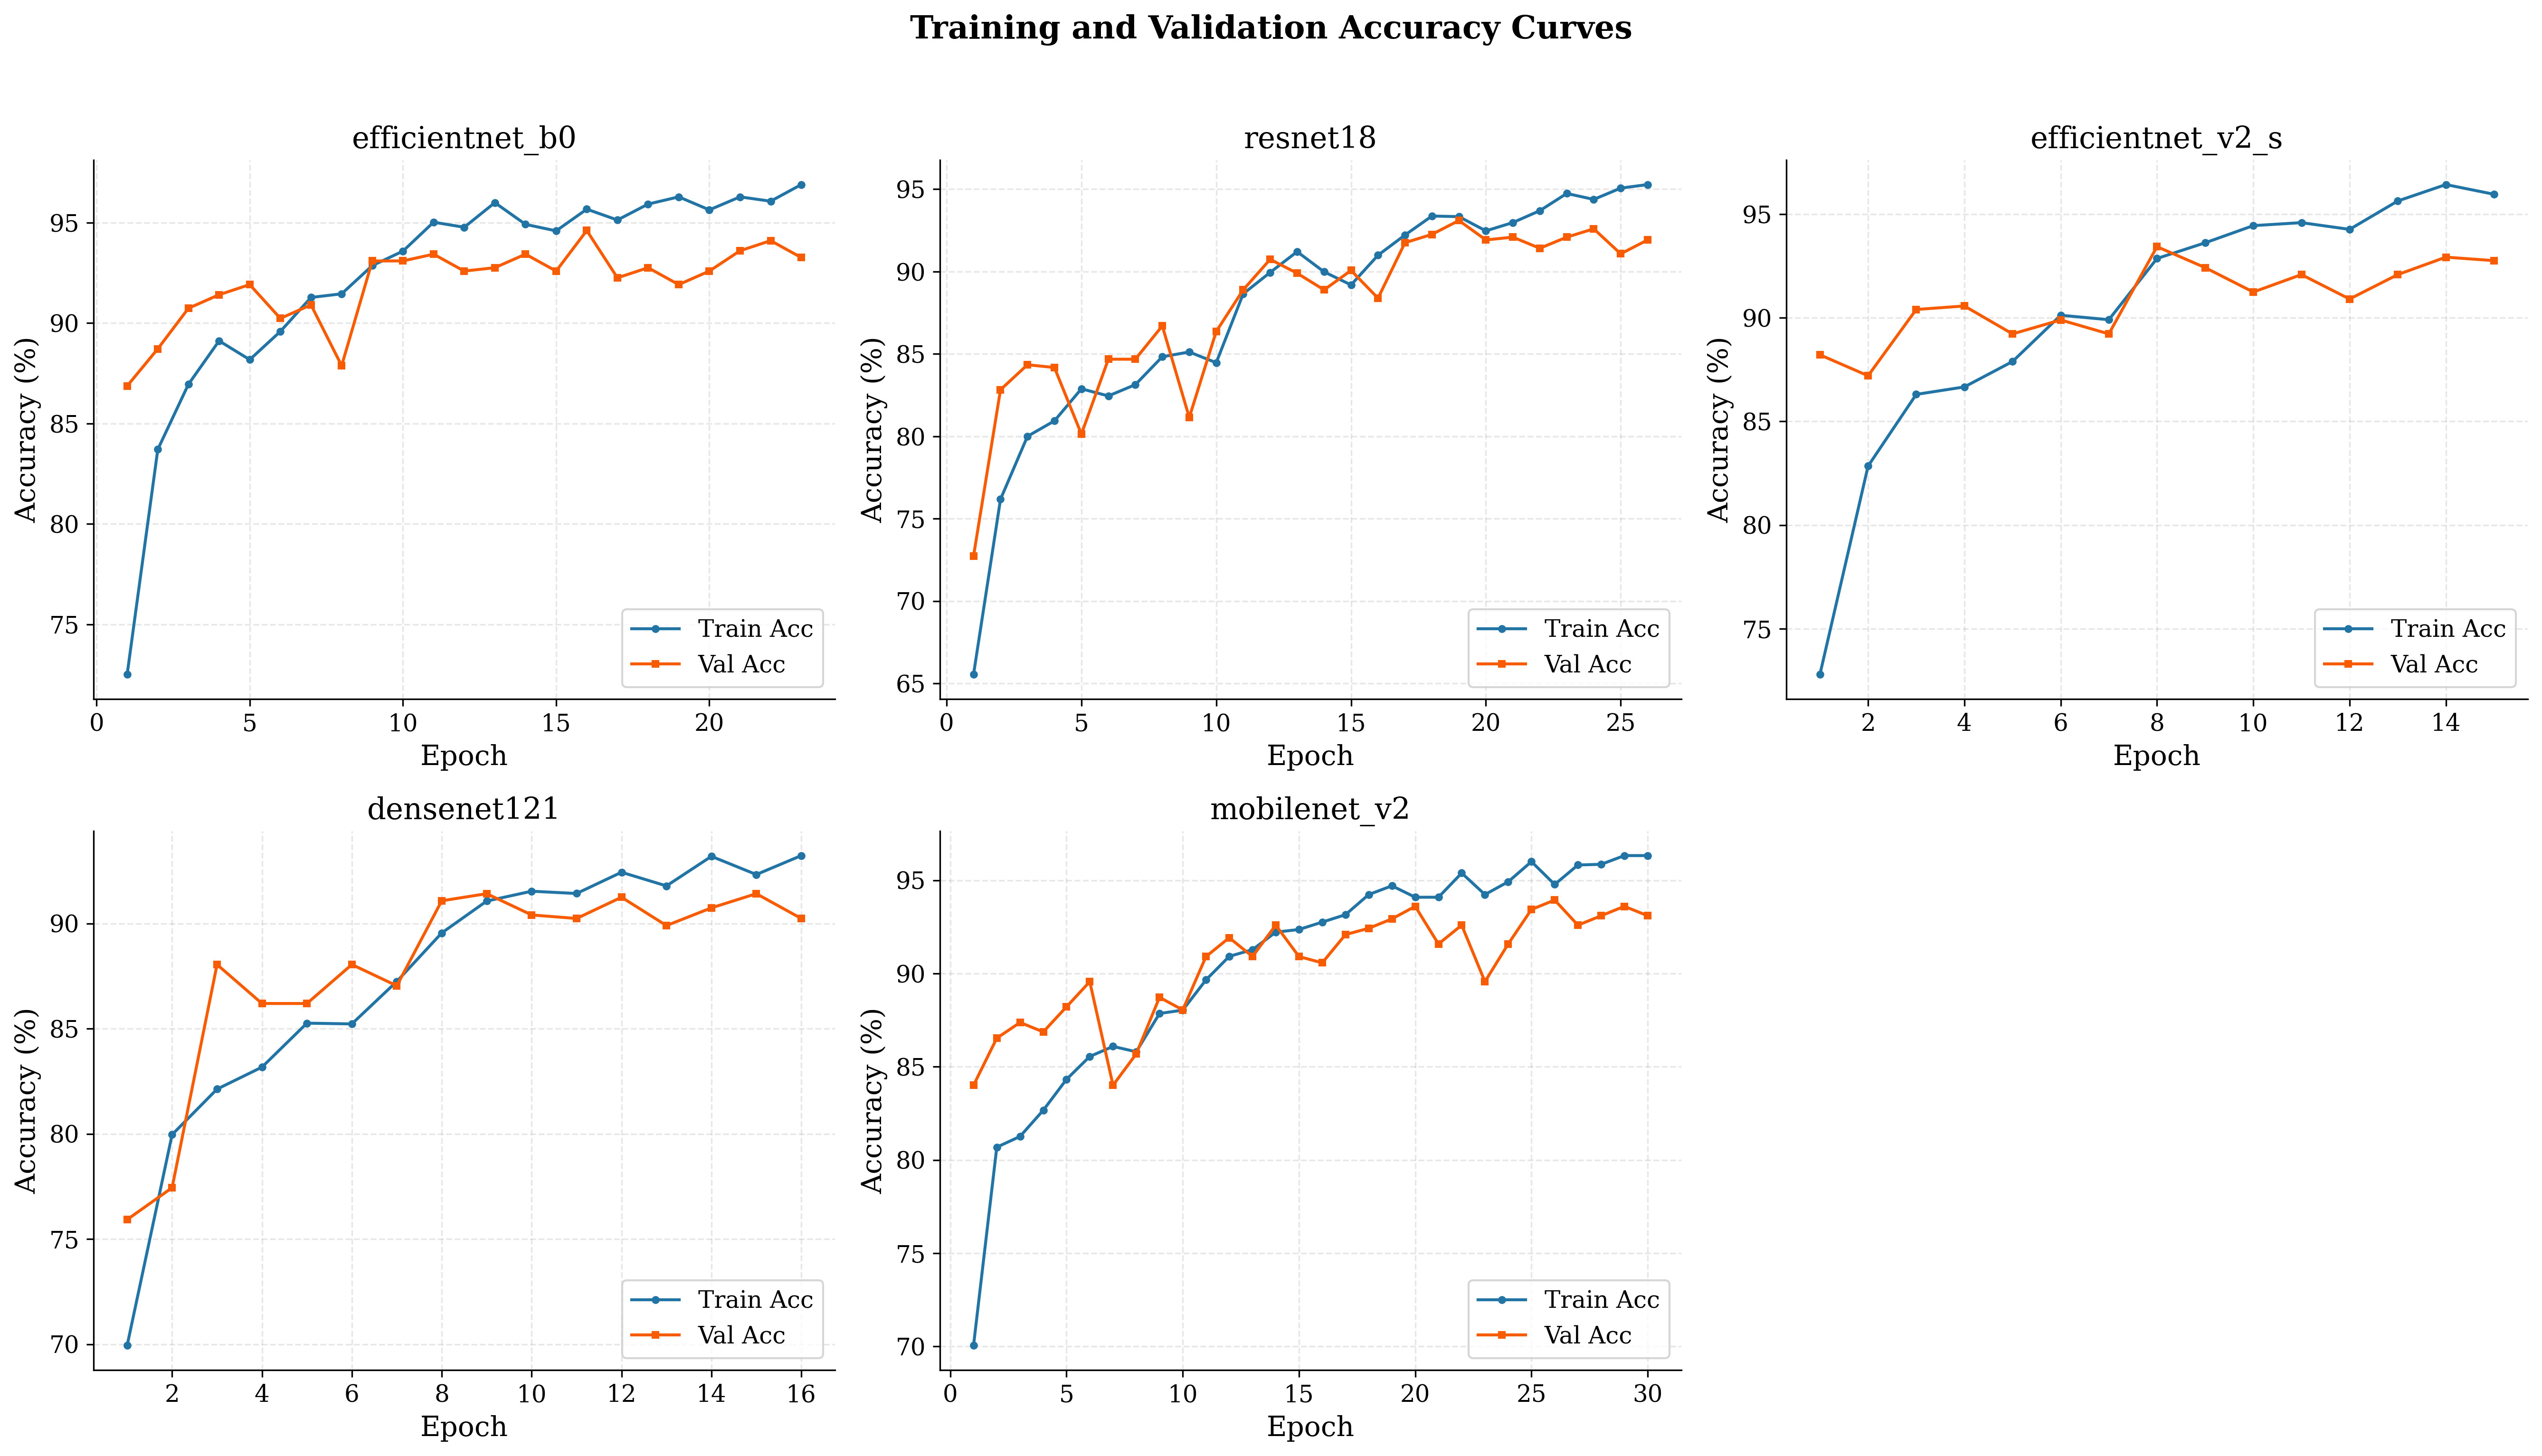
\includegraphics[width=\textwidth]{fig_accuracy_curves.jpg}}
\caption{Training and validation accuracy curves for the five evaluated architectures on the BD3 dataset. Rapid convergence and a small train--validation gap are visible across all models.}
\label{fig:acc_curves}
\end{figure*}

\subsection{Per-Class Performance}
Table~\ref{tab:classification_report} reports the per-class precision, recall, and F1-score for the best model, EfficientNet-B0. The \textit{plain} and \textit{algae} classes are the easiest to recognize (F1 of 0.994 and 0.981, respectively), whereas the \textit{major\_crack} class is the most challenging (F1 of 0.887), reflecting its visual overlap with \textit{minor\_crack}. Fig.~\ref{fig:f1_heatmap} extends this analysis across all models, confirming that the relative class difficulty is consistent: every architecture finds \textit{plain} and \textit{algae} easiest and the two crack-severity classes hardest.

\begin{table}[htbp]
\caption{Per-Class Performance of EfficientNet-B0 on the Test Set}
\label{tab:classification_report}
\centering
\begin{tabular}{lcccc}
\toprule
\textbf{Class} & \textbf{Precision} & \textbf{Recall} & \textbf{F1} & \textbf{Support} \\
\midrule
algae        & 0.975 & 0.987 & 0.981 & 78 \\
major\_crack & 0.874 & 0.900 & 0.887 & 100 \\
minor\_crack & 0.914 & 0.895 & 0.904 & 95 \\
peeling      & 0.952 & 0.882 & 0.916 & 68 \\
plain        & 0.989 & 1.000 & 0.994 & 86 \\
spalling     & 0.892 & 0.937 & 0.914 & 79 \\
stain        & 0.966 & 0.944 & 0.955 & 90 \\
\midrule
\textbf{Macro avg}    & 0.937 & 0.935 & 0.936 & 596 \\
\textbf{Weighted avg} & 0.935 & 0.935 & 0.935 & 596 \\
\bottomrule
\end{tabular}
\end{table}

\begin{figure}[htbp]
\centerline{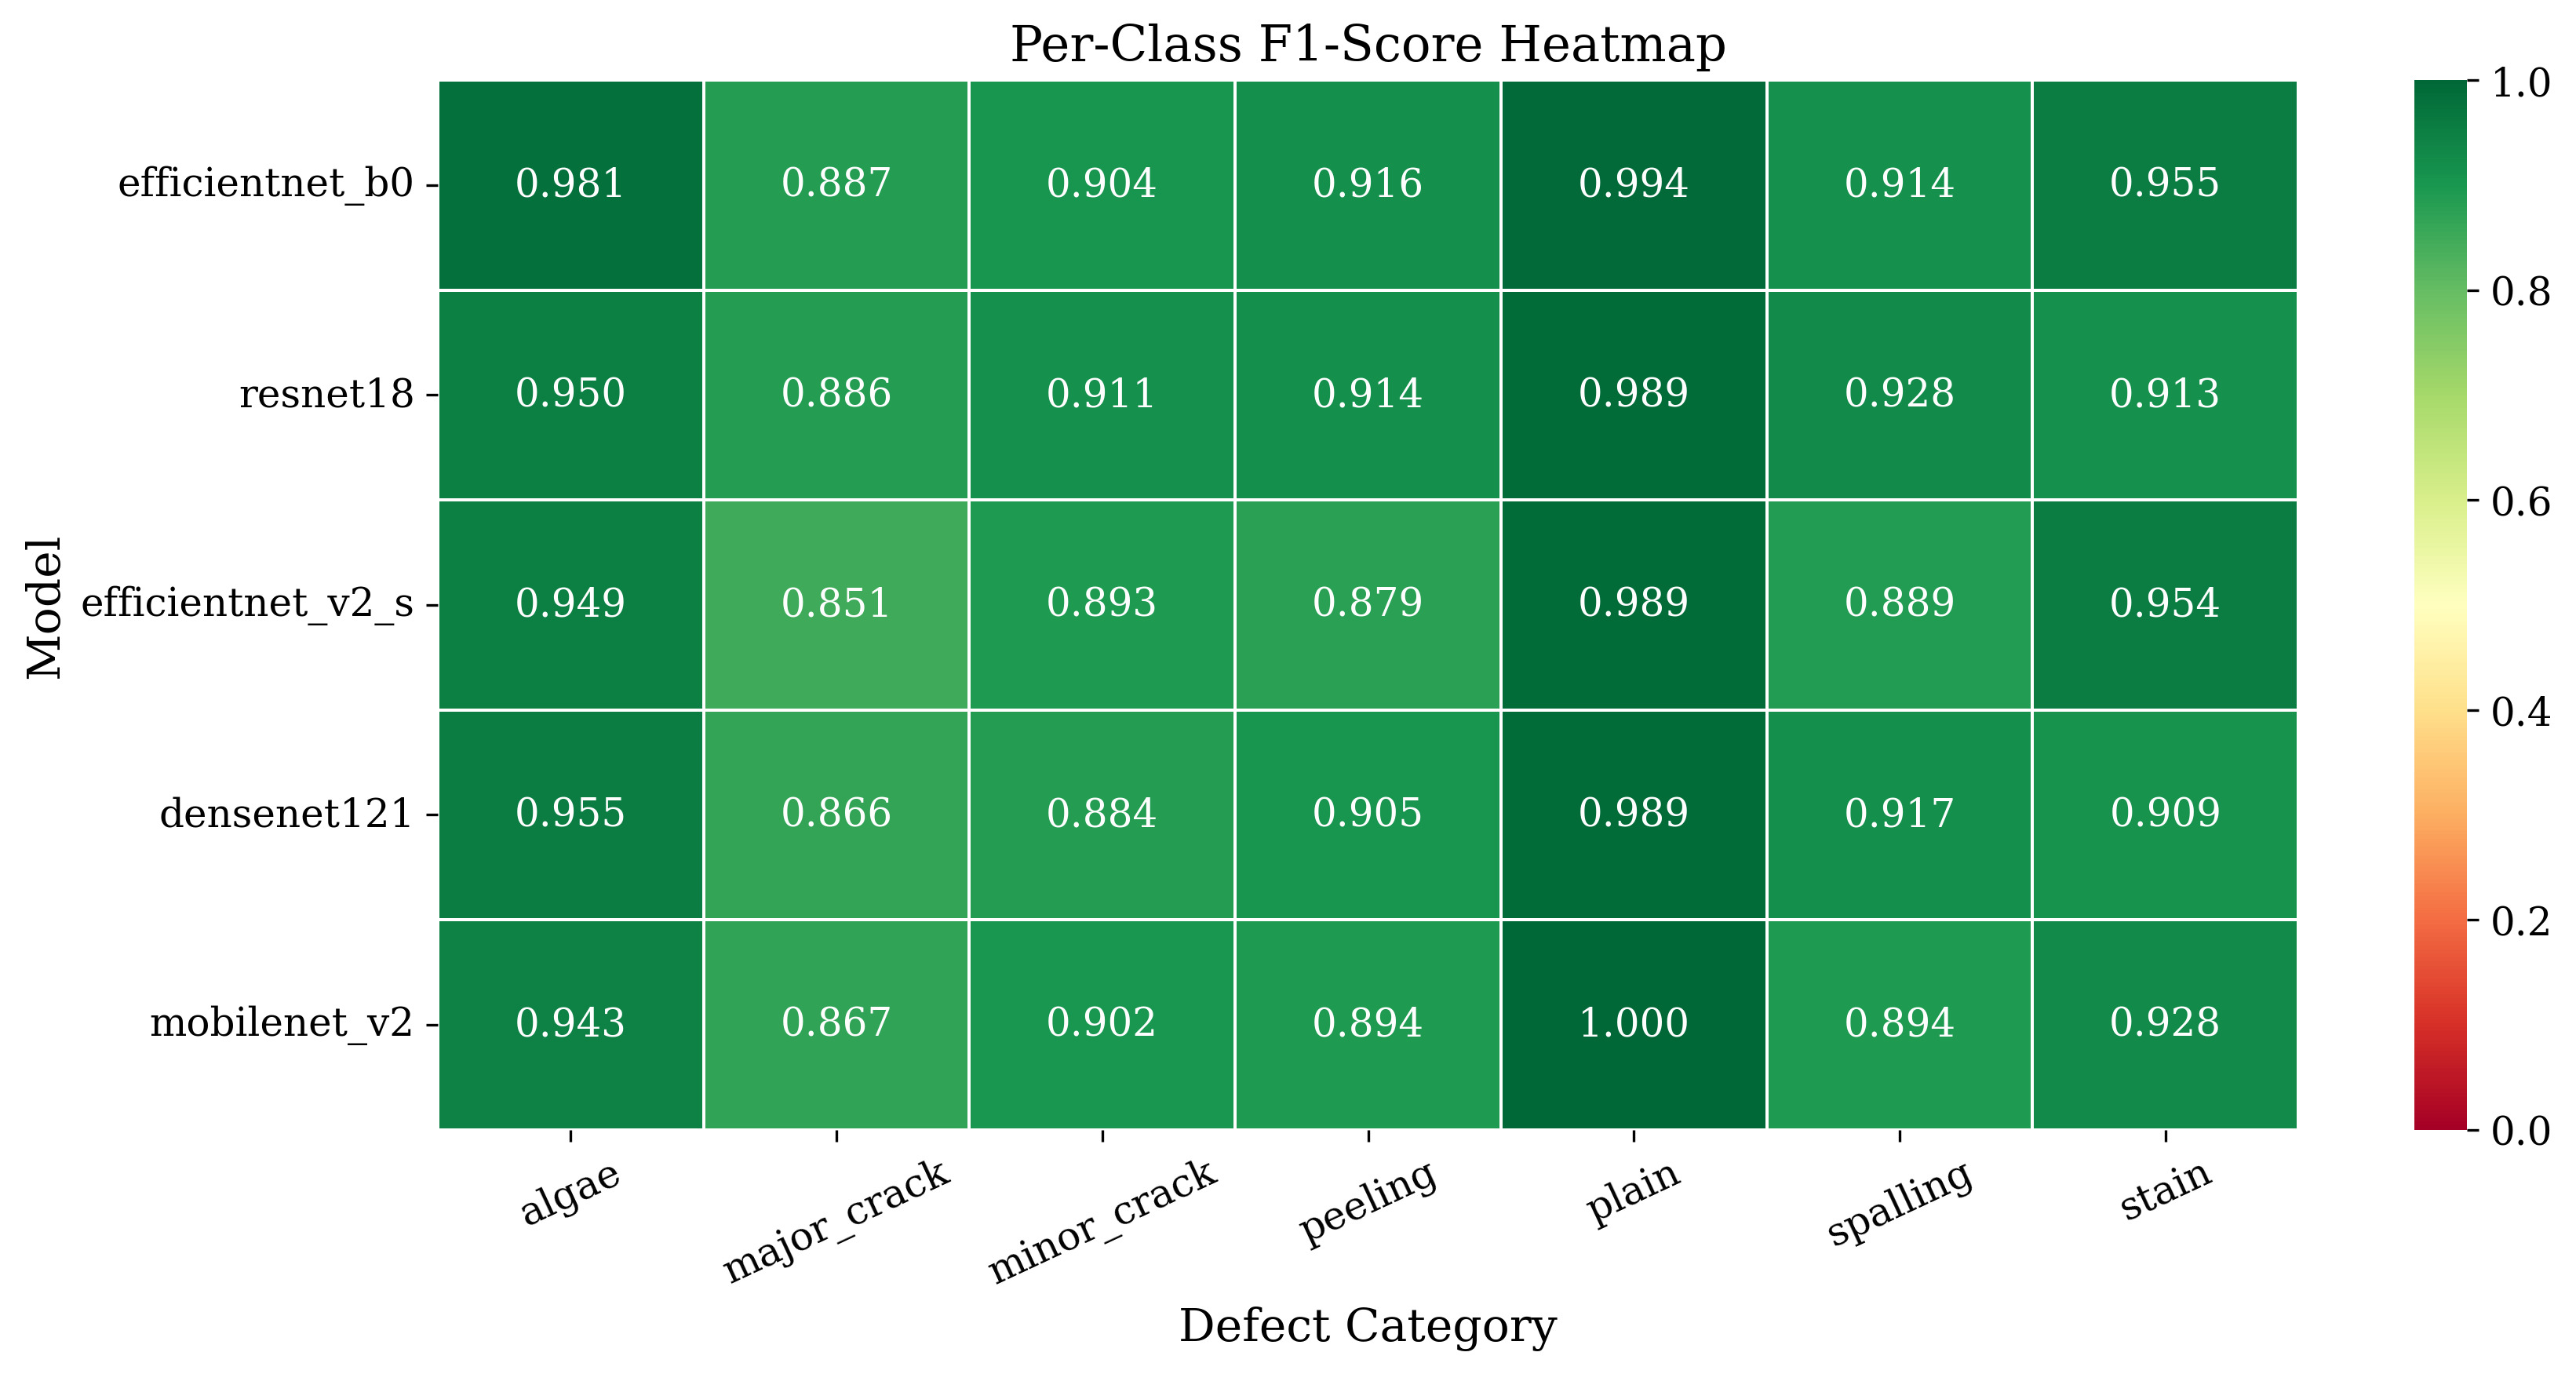
\includegraphics[width=\linewidth]{heatmap.jpg}}
\caption{Per-class F1-score heatmap across all five models and seven defect classes on the BD3 test set.}
\label{fig:f1_heatmap}
\end{figure}

\subsection{Confusion Analysis}
Fig.~\ref{fig:confusion} presents the row-normalized confusion matrices for all five models. Two systematic error modes are visible across architectures. The dominant confusion is between \textit{major\_crack} and \textit{minor\_crack}: for EfficientNet-B0, 8 of 100 \textit{major\_crack} samples were predicted as \textit{minor\_crack}, and 7 of 95 \textit{minor\_crack} samples as \textit{major\_crack}. The second confusion is between \textit{peeling} and \textit{spalling}, which share overlapping surface texture and frequently co-occur on the same wall. The \textit{plain} class incurred no misclassifications for the best model (86/86 correct).

\begin{figure*}[t]
\centerline{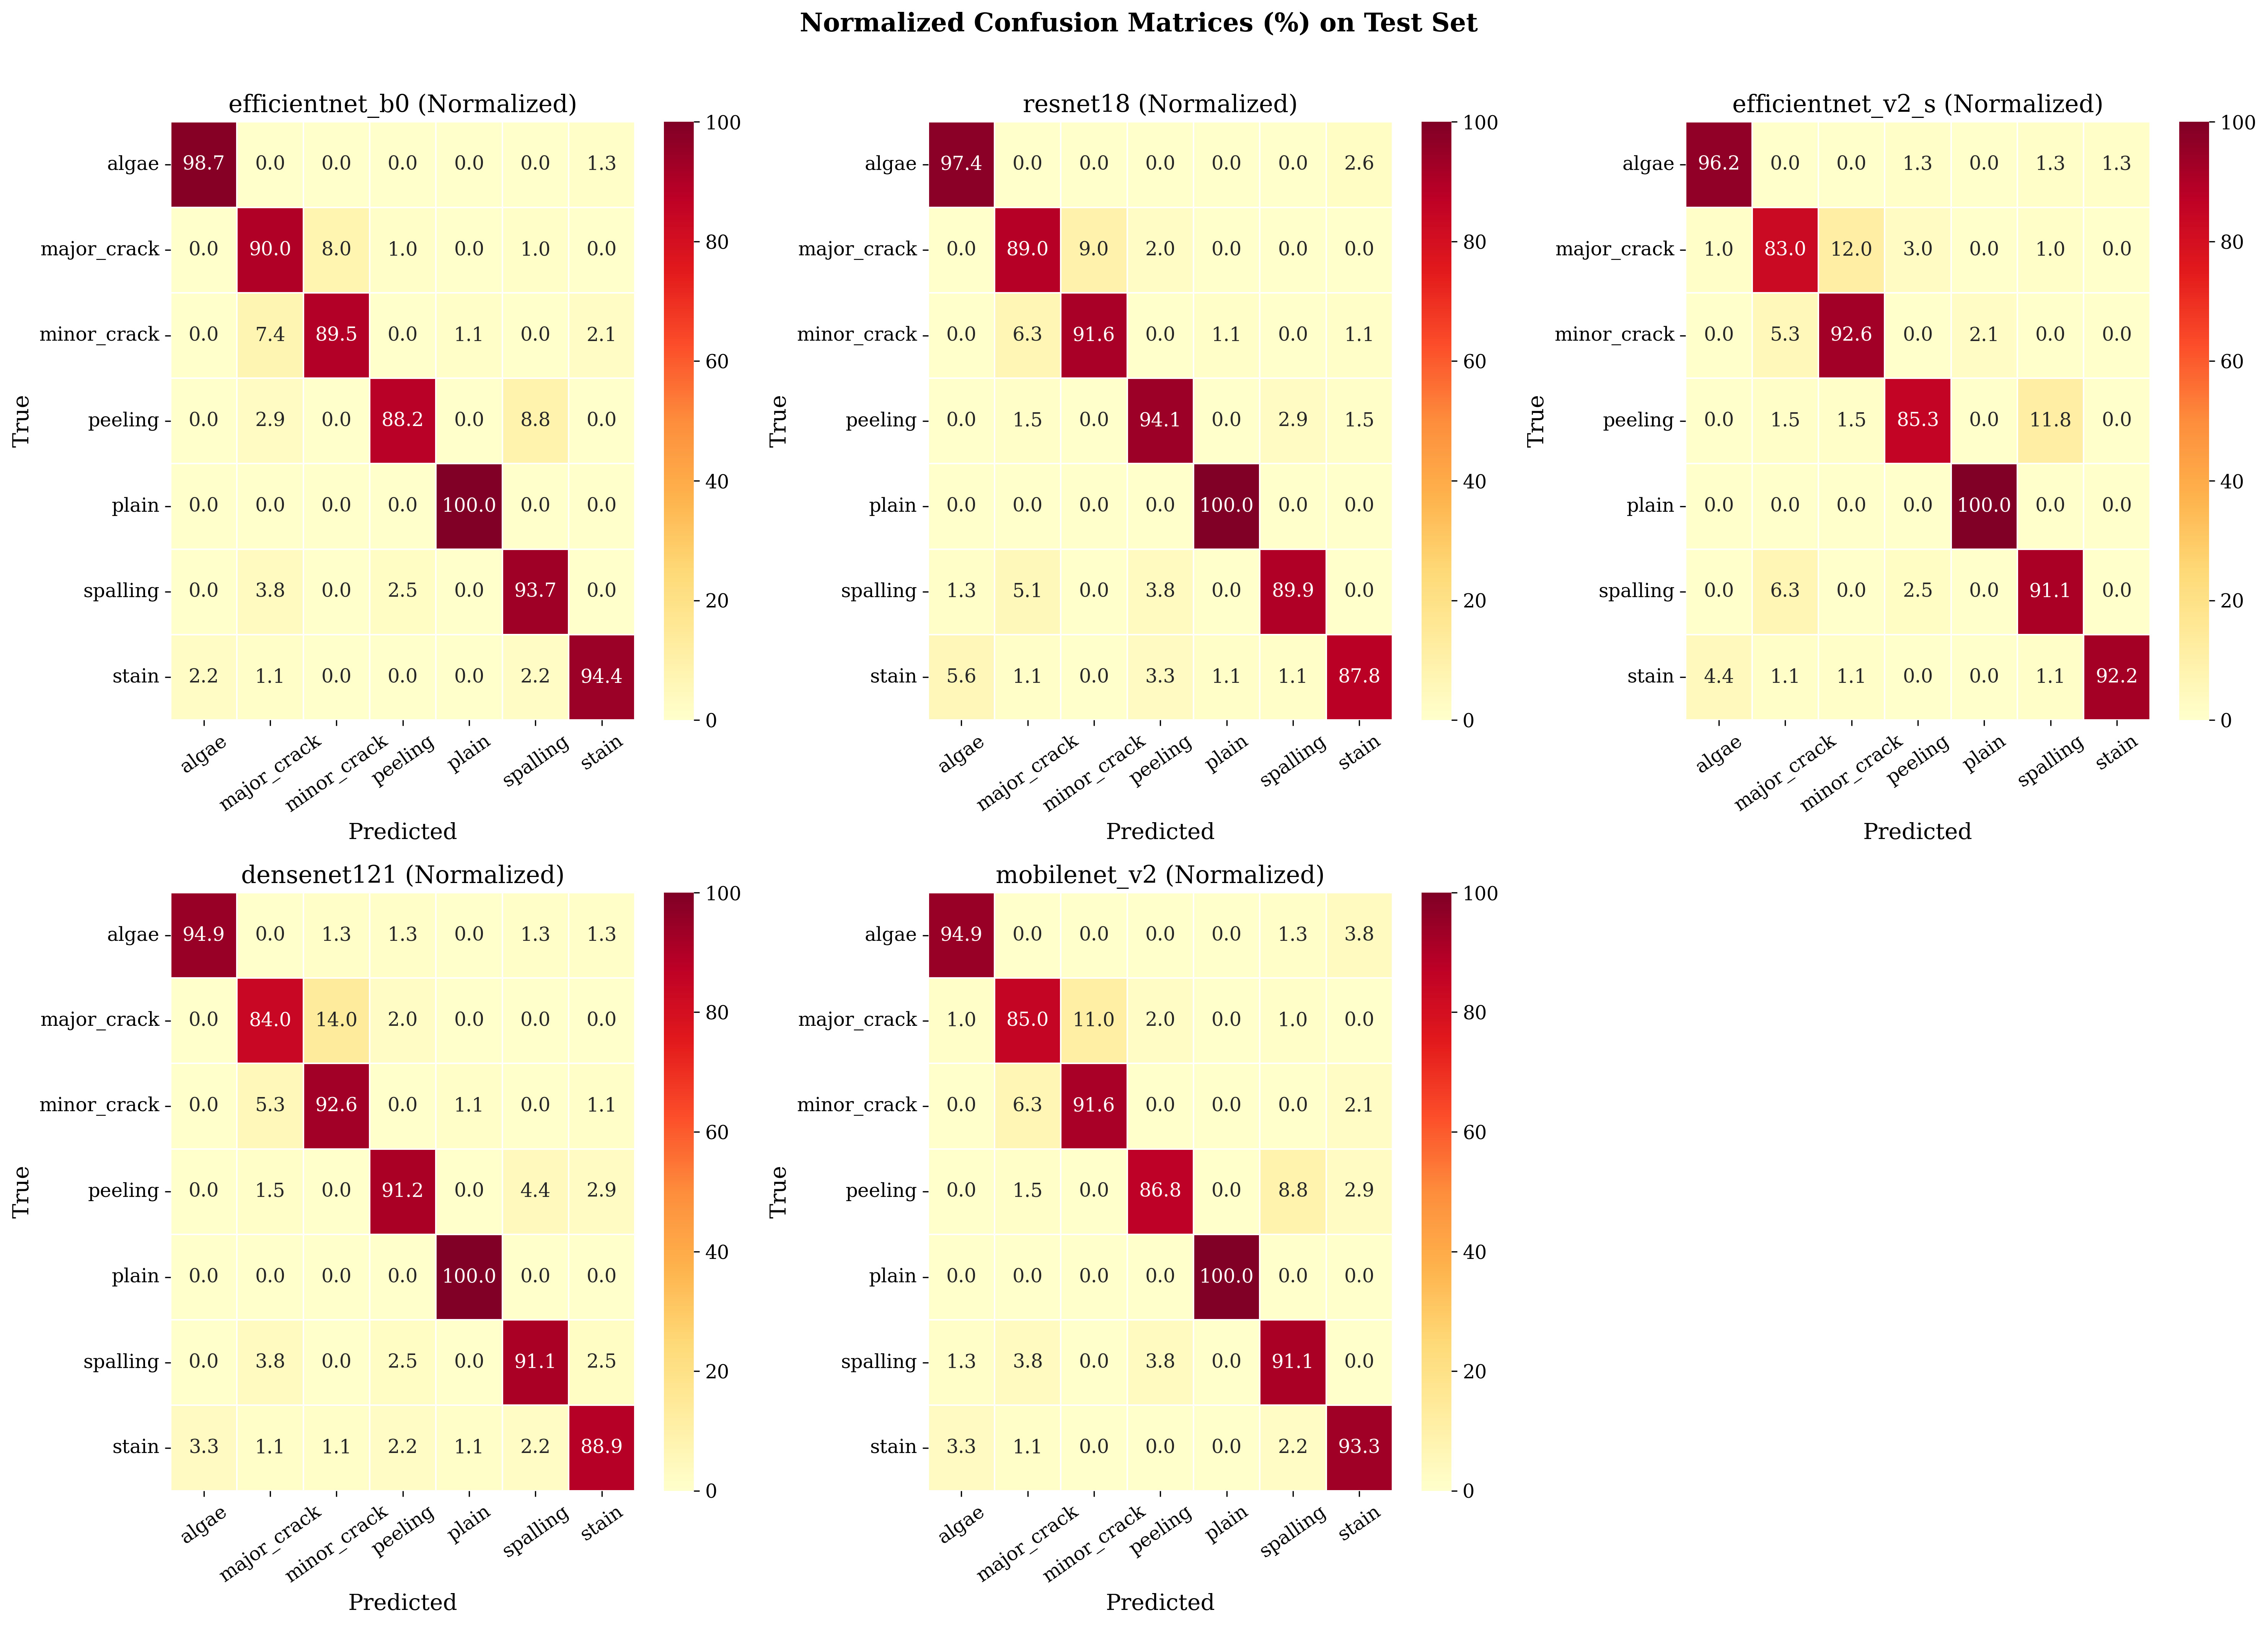
\includegraphics[width=\textwidth]{fig_confusion_norm.jpg}}
\caption{Row-normalized confusion matrices (\%) on the BD3 test set for all five architectures.}
\label{fig:confusion}
\end{figure*}

\subsection{ROC and Precision--Recall Analysis}
The one-versus-rest ROC curves for EfficientNet-B0 are shown in Fig.~\ref{fig:roc}, and the per-class AUC and AP values are summarized in Table~\ref{tab:roc_ap}. The model attains near-perfect ranking, with all classes achieving an AUC of at least 0.987 and a macro-average AUC of approximately 0.994. The \textit{plain} class is perfectly separable (AUC 1.000, AP 1.000), and even the most difficult \textit{major\_crack} class achieves an AUC of 0.987. The corresponding precision--recall curves are shown in Fig.~\ref{fig:pr}; the high average-precision values confirm robust behavior across decision thresholds, including for the harder \textit{peeling} and \textit{spalling} classes. The consistently high AUC indicates reliable probability ranking, an important property for automated triage where defects are prioritized by predicted severity.

\begin{table}[htbp]
\caption{Per-Class ROC AUC and Average Precision for EfficientNet-B0}
\label{tab:roc_ap}
\centering
\begin{tabular}{lcc}
\toprule
\textbf{Class} & \textbf{ROC AUC} & \textbf{AP} \\
\midrule
algae        & 0.999 & 0.995 \\
major\_crack & 0.987 & 0.943 \\
minor\_crack & 0.990 & 0.954 \\
peeling      & 0.991 & 0.935 \\
plain        & 1.000 & 1.000 \\
spalling     & 0.991 & 0.966 \\
stain        & 0.996 & 0.985 \\
\bottomrule
\end{tabular}
\end{table}

\begin{figure}[htbp]
\centerline{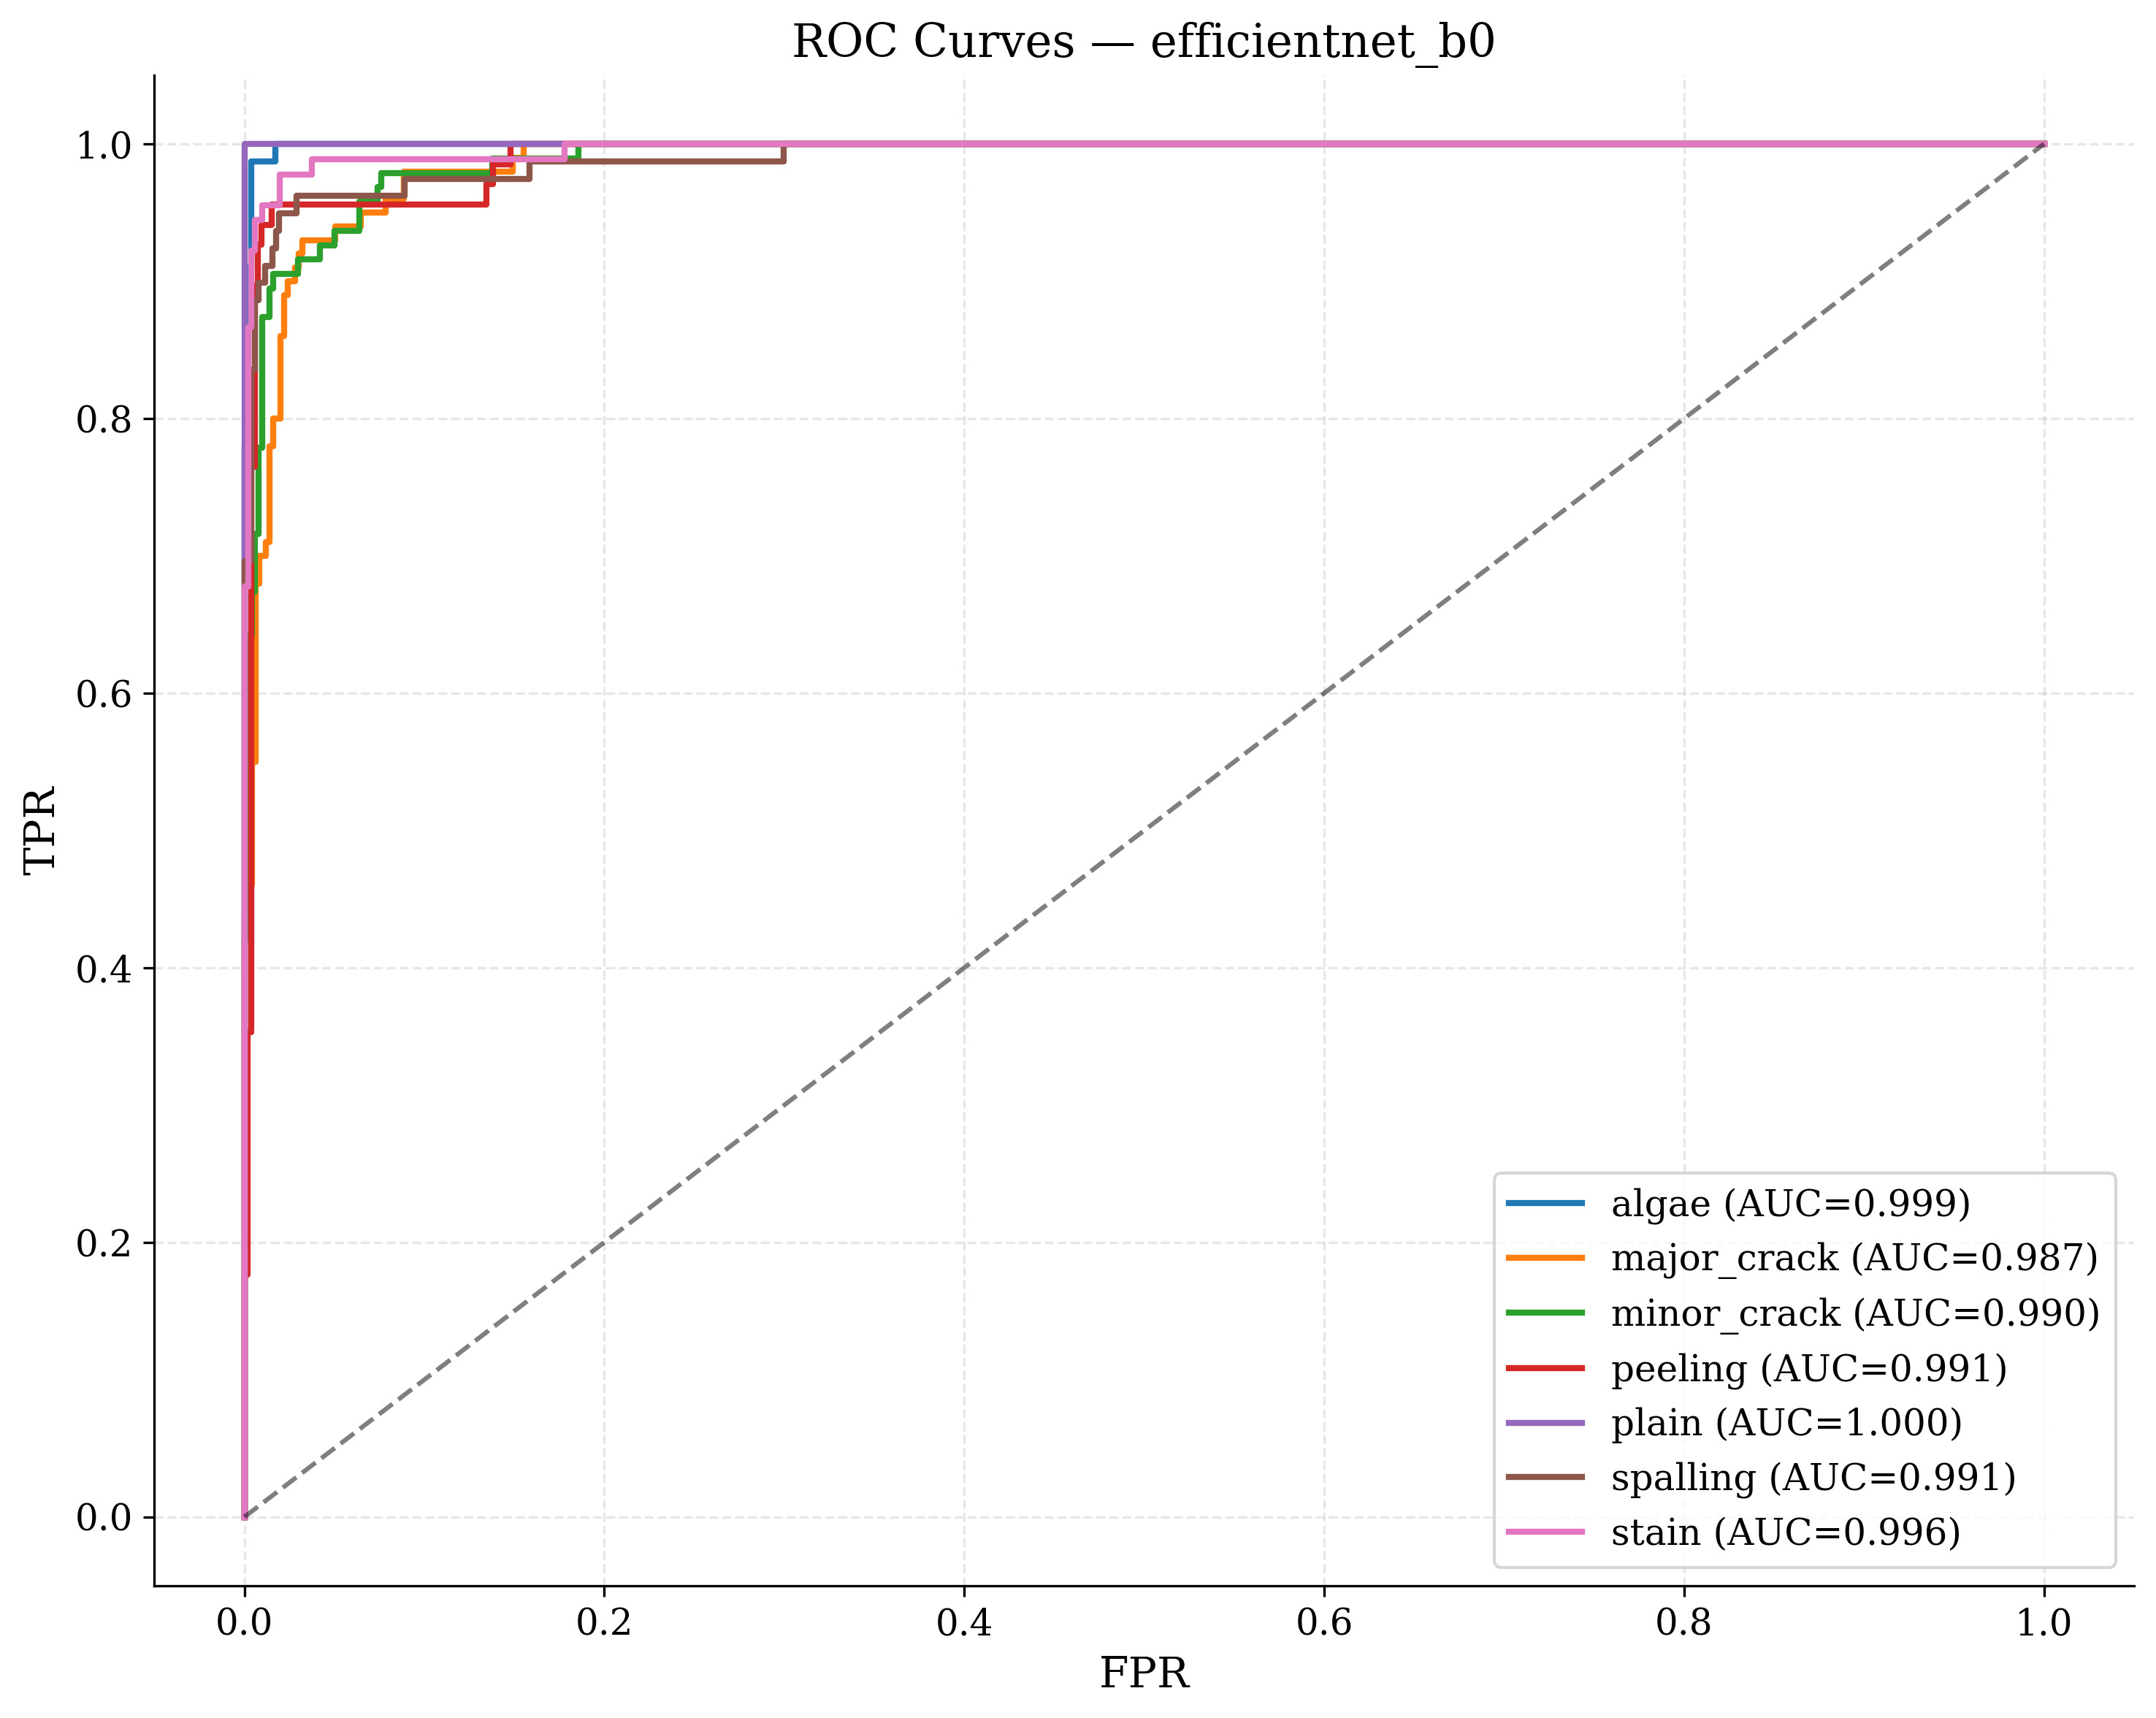
\includegraphics[width=\linewidth]{roc.jpg}}
\caption{One-versus-rest ROC curves for EfficientNet-B0 across the seven defect classes (BD3 test set).}
\label{fig:roc}
\end{figure}

\begin{figure}[htbp]
\centerline{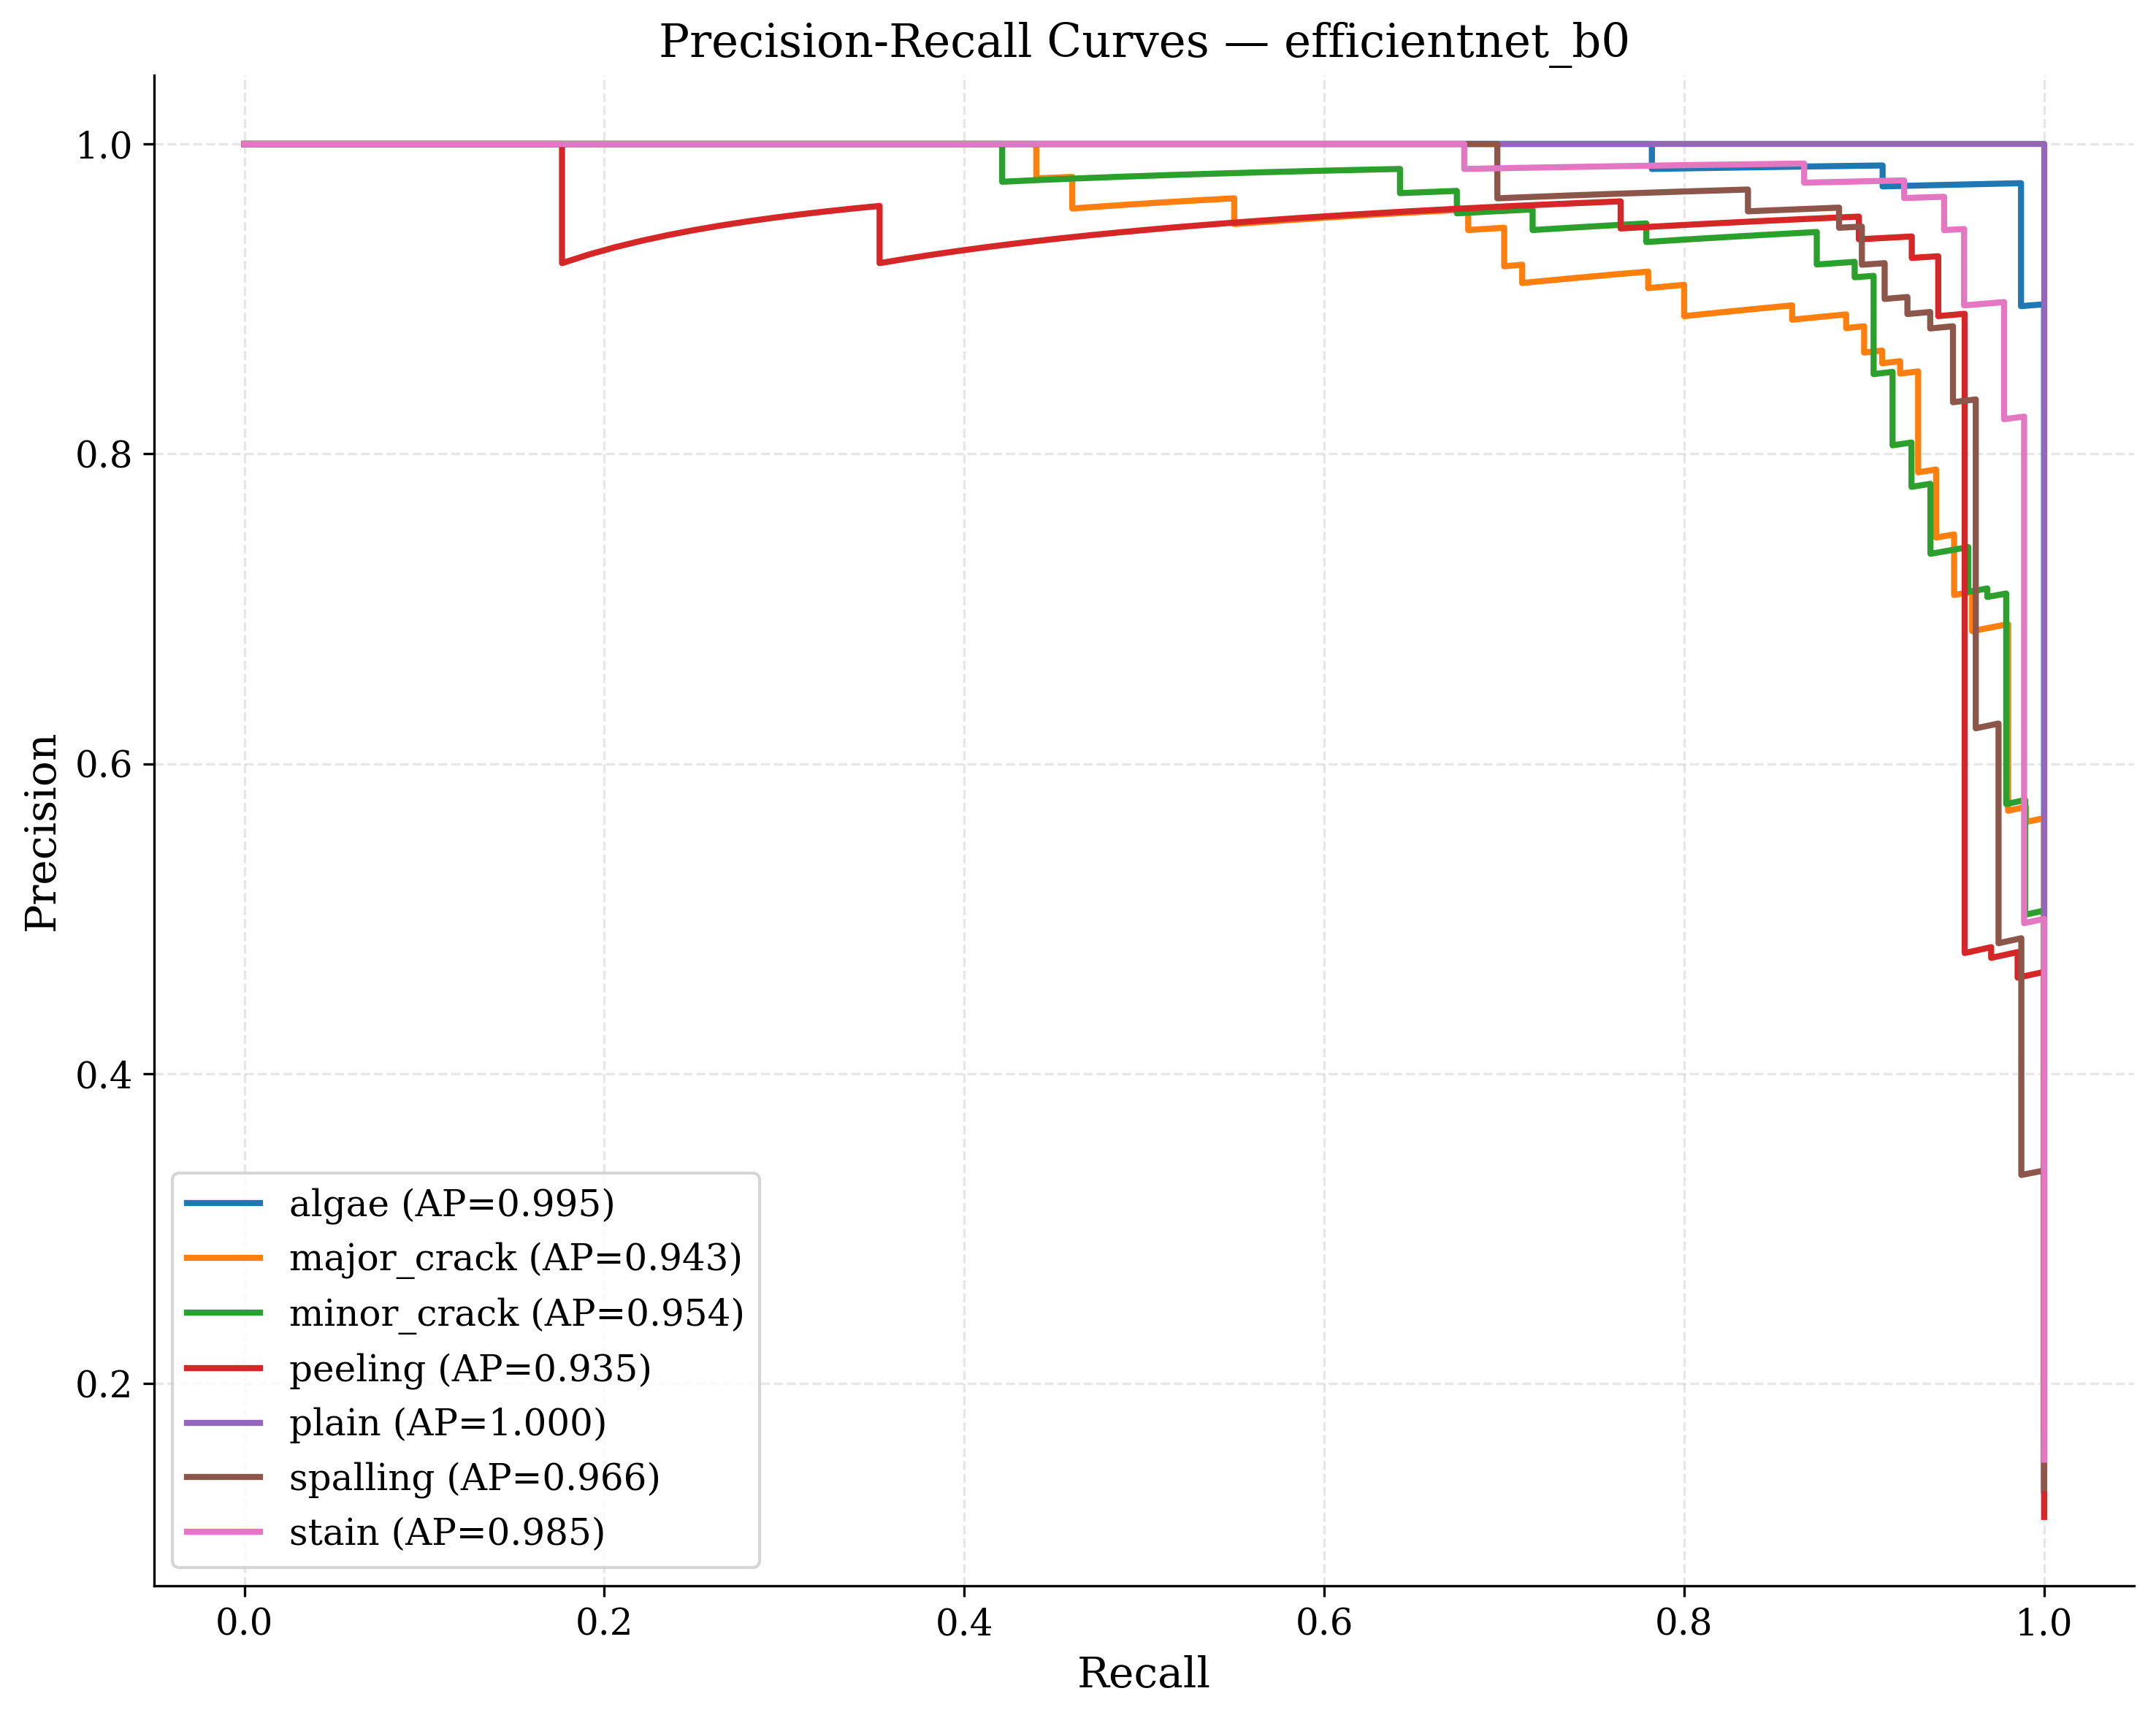
\includegraphics[width=\linewidth]{fig_pr_curves.jpg}}
\caption{Precision--recall curves for EfficientNet-B0 across the seven defect classes; per-class average precision (AP) is listed in Table~\ref{tab:roc_ap}.}
\label{fig:pr}
\end{figure}

\subsection{Comparison with Existing Methods}
\label{sec:comparison}
Table~\ref{tab:comparison} situates our results against prior work, most importantly the original BD3 benchmark~\cite{ref40}, which evaluated five classifiers on the same dataset. This comparison must be read with care: \cite{ref40} uses its own train/test split and reports results both without augmentation and with a fixed offline expansion of the training set to roughly 14{,}000 images, whereas the present study uses a 70/15/15 split with on-the-fly augmentation. The numbers are therefore indicative rather than split-matched. Under BD3's non-augmented setting, the best reported model is a Vision Transformer (ViT) at macro-F1 0.932; our EfficientNet-B0 reaches 0.936, i.e., on par with that ViT---and within single-run sampling noise of it---while using roughly an order of magnitude fewer parameters (4.02M versus a ViT-Base-scale $\approx$86M). Under BD3's augmented setting, however, its ViT (0.988) and ResNet-18 (0.971) exceed our scores; we therefore claim parameter-efficiency parity, not state-of-the-art accuracy. We further observe that the lightweight backbones reach substantially higher macro-F1 under our protocol than the non-augmented values in~\cite{ref40} (e.g., ResNet-18 0.927 vs 0.830; MobileNet-V2 0.918 vs 0.842). Because split, augmentation, and random seed all differ between the two studies, this observation is consistent with---but does not by itself establish---a strong influence of the training protocol relative to raw capacity; a controlled within-study augmentation ablation is left to future work. For broader context, the table also lists representative multi-class defect classifiers on \emph{other} datasets and tasks; these use different data and metrics and are included only to indicate the typical performance range.

\begin{table*}[t]
\caption{Comparison with Prior Building, Facade, and Concrete Defect Classification Methods. BD3~\cite{ref40} uses its own train/test split and reports macro-F1 without\,/\,with a fixed offline training-set augmentation ($\approx$14k images), so its values are indicative rather than split-matched. Parameter counts marked $\approx$ are nominal (ViT-Base, AlexNet, and VGG-16 scales). The ``other datasets'' block uses different data, class sets, and metrics and is contextual only.}
\label{tab:comparison}
\centering
\begin{tabular}{llcc}
\toprule
\textbf{Method} & \textbf{Params (M)} & \textbf{Macro-F1 (no aug.\,/\,aug.)} & \textbf{Test Acc (\%)} \\
\midrule
\multicolumn{4}{l}{\textit{BD3 benchmark~\cite{ref40} --- same dataset, BD3's own split and protocol}}\\
Vision Transformer~\cite{ref40} & $\approx$86  & 0.932\,/\,0.988 & --- \\
AlexNet~\cite{ref40}            & $\approx$61  & 0.880\,/\,0.939 & --- \\
VGG-16~\cite{ref40}             & $\approx$138 & 0.836\,/\,0.906 & --- \\
ResNet-18~\cite{ref40}          & 11.7         & 0.830\,/\,0.971 & --- \\
MobileNet-V2~\cite{ref40}       & 3.5          & 0.842\,/\,0.875 & --- \\
\midrule
\multicolumn{4}{l}{\textit{This work --- 70/15/15 split, on-the-fly augmentation}}\\
\textbf{EfficientNet-B0}        & \textbf{4.02}  & \textbf{0.936} & \textbf{93.46} \\
ResNet-18                       & 11.18          & 0.927 & 92.62 \\
MobileNet-V2                    & 2.23           & 0.918 & 91.78 \\
\midrule
\multicolumn{4}{l}{\textit{Other datasets and tasks --- contextual reference only}}\\
Perez \textit{et al.}~\cite{ref9} (VGG-16), building, 4-class  & $\approx$138 & --- & 87.50 \\
Guo \textit{et al.}~\cite{ref10} (meta-CNN), facade, multi-class & ---        & --- & 82.86 \\
Mundt \textit{et al.}~\cite{ref11} (CODEBRIM), concrete, 6-class & ---        & --- & $\approx$72$^{*}$ \\
\bottomrule
\end{tabular}
\\[2pt]
{\footnotesize $^{*}$Multi-target accuracy (all defect labels per image correct); not directly comparable to single-label top-1 accuracy.}
\end{table*}

\section{Discussion}

\subsection{Performance Strengths and Model Efficacy}
The results underscore the efficacy of transfer learning for structural-defect classification. All models converged rapidly, with EfficientNet-B0 reaching 86.87\% validation accuracy within a single epoch, confirming that ImageNet feature representations transfer well to the textural domain of building materials. The comprehensive augmentation strategy effectively mitigated overfitting: as shown in Fig.~\ref{fig:overfit}, the generalization gap between training and validation accuracy remained small across all architectures throughout training. At the system level, the framework achieved a macro-average AUC of at least 0.993 for every model, indicating reliable probability ranking---a prerequisite for automated triage in real-world inspection pipelines. Most importantly, the comparison in Table~\ref{tab:comparison} shows that a compact EfficientNet-B0 reaches a macro-F1 on par with a Vision Transformer of roughly an order of magnitude more parameters under BD3's non-augmented setting. We frame this as parameter efficiency rather than superiority: BD3's augmented runs achieve higher F1, and the cross-paper comparison is confounded by differing splits and augmentation. The consistent strength of lightweight backbones under our protocol is suggestive of a substantial role for transfer learning and augmentation relative to raw capacity, but establishing this causally would require a controlled within-study ablation.

\begin{figure}[htbp]
\centerline{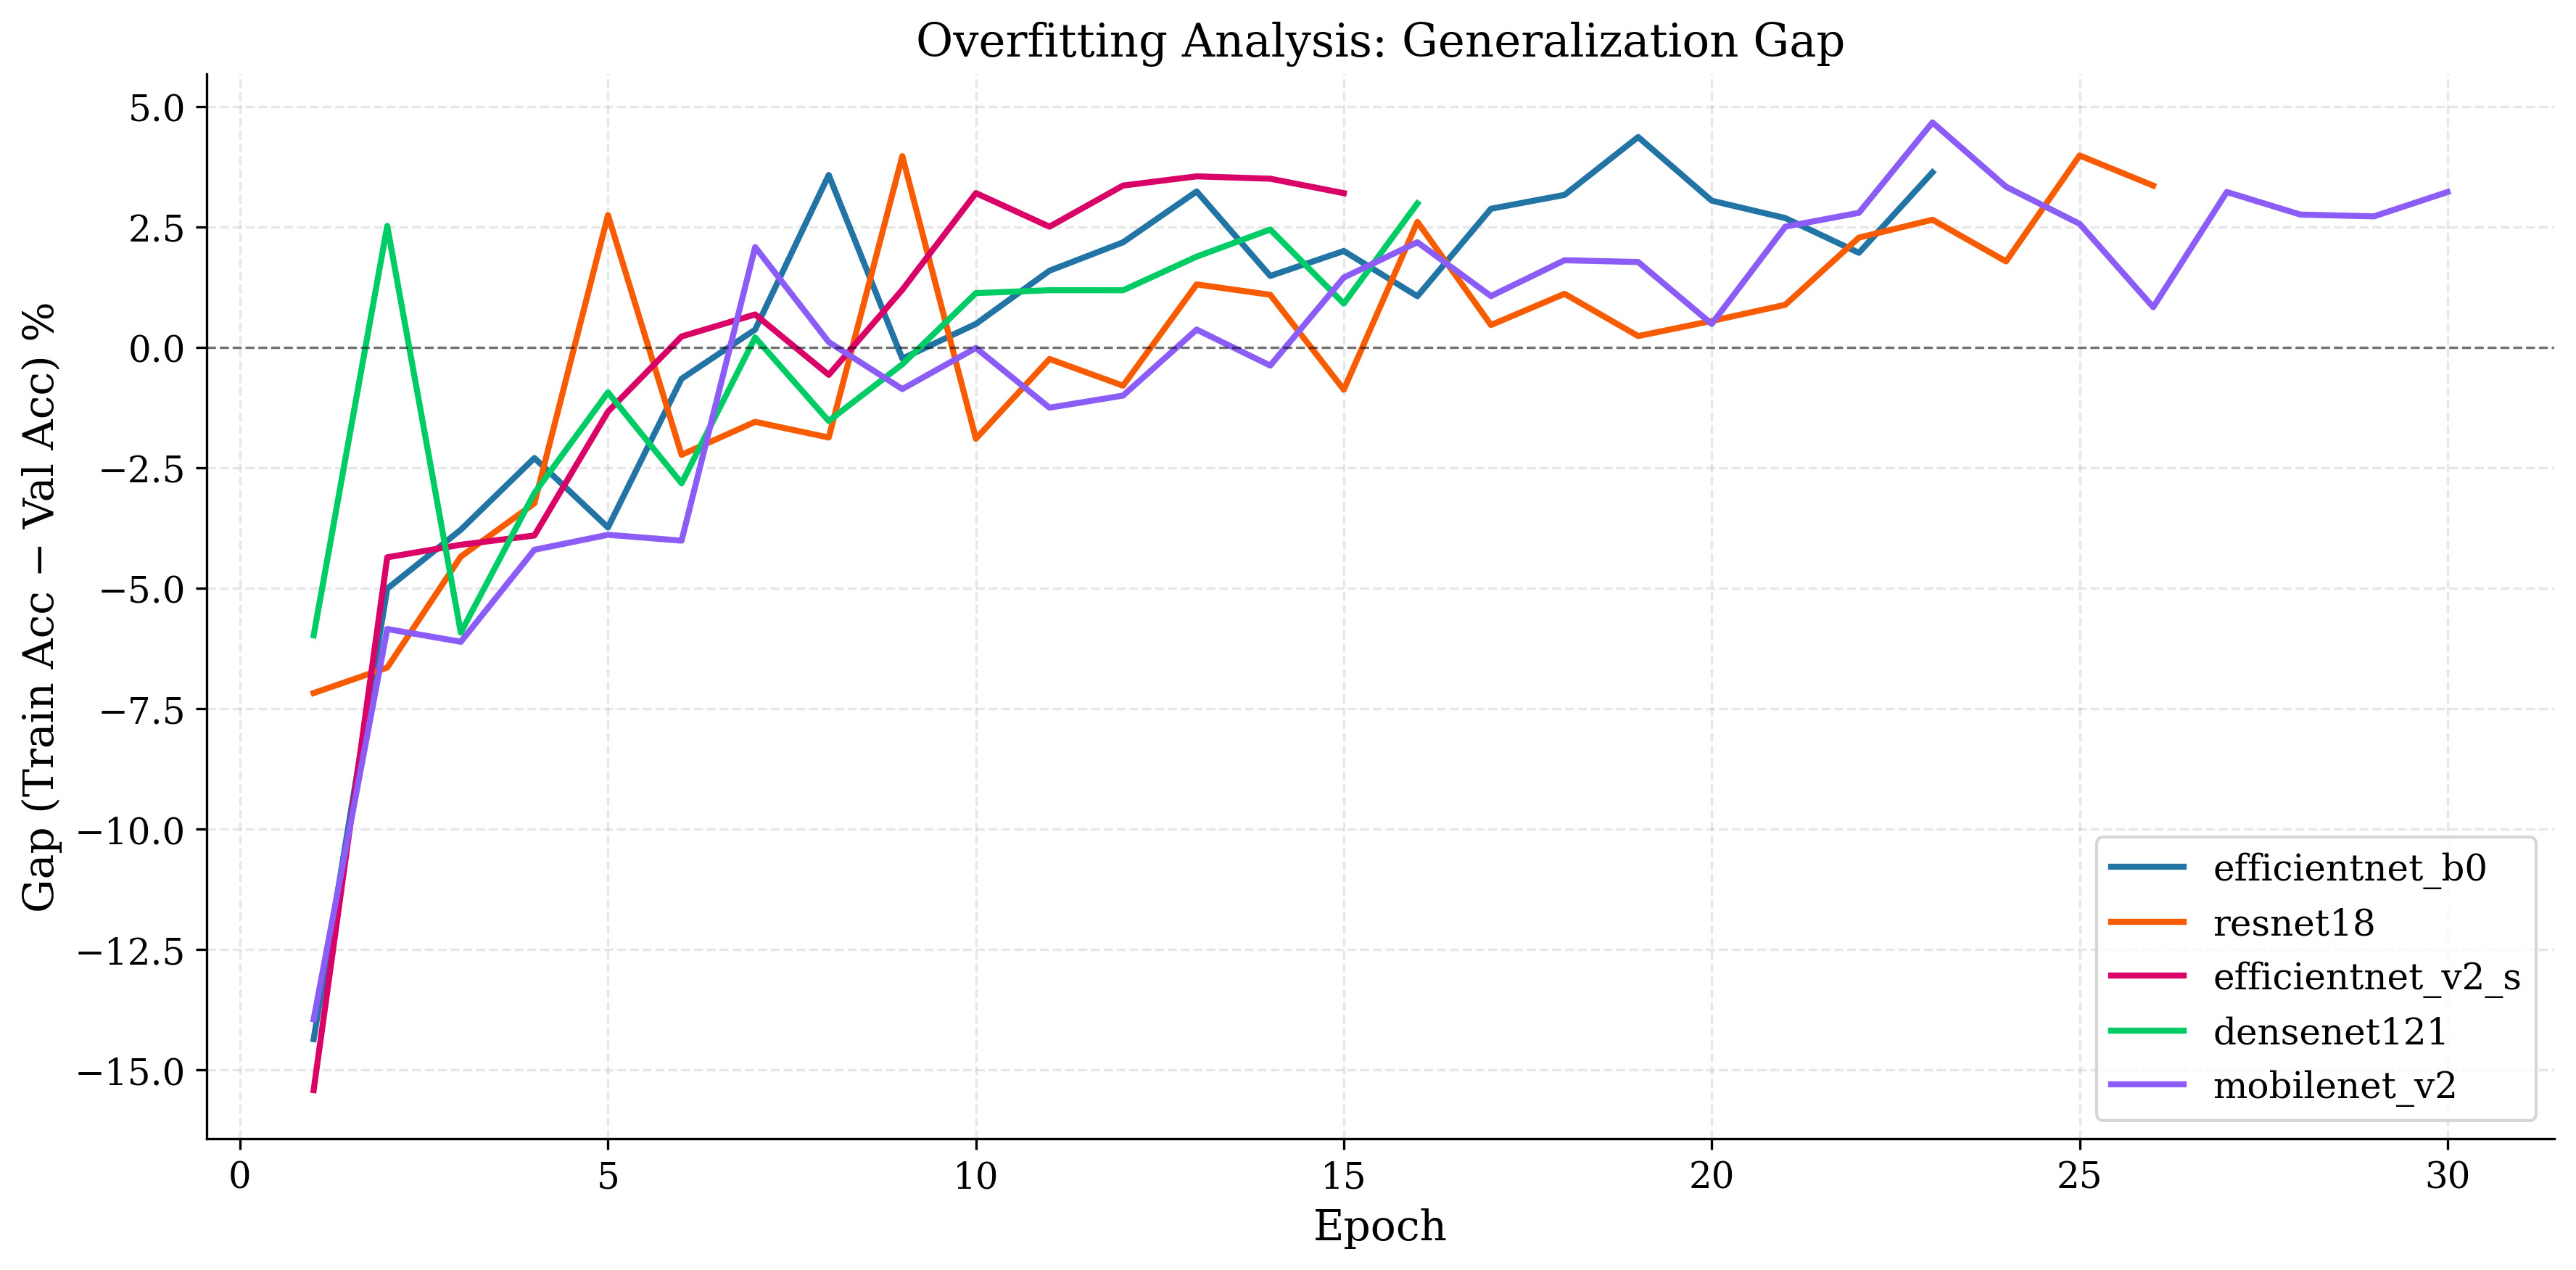
\includegraphics[width=\linewidth]{fig_overfitting_gap.jpg}}
\caption{Generalization gap (training accuracy minus validation accuracy) per epoch for all five models on the BD3 dataset. The gap remains small throughout training, indicating limited overfitting.}
\label{fig:overfit}
\end{figure}

\subsection{Limitations and Challenges}
\label{sec:limitations}
Several limitations temper these results. First, the most frequent misclassification, between \textit{major\_crack} and \textit{minor\_crack}, reflects an inherent ambiguity in crack-severity labeling that often requires expert judgment even for human annotators; the boundary between severity grades is not sharply defined visually. Cross-class confusion between \textit{peeling} and \textit{spalling} similarly arises from their overlapping texture and frequent co-location on the same surface. Second, although the BD3 dataset spans both heritage and ordinary facades, it is not exclusively heritage-specific; consequently, the present study should be read as evidence that the approach is \emph{applicable} to heritage inspection rather than as a heritage-only validation, and dedicated evaluation on curated heritage imagery remains important future work. Third, the evaluation is single-run: although a fixed seed ensures reproducibility, the reported test accuracies carry $\pm2$-point confidence intervals that overlap across models, so the architecture ranking is indicative rather than definitive, and reporting variance across multiple seeds or cross-validation folds would strengthen the statistical claims. The same single-run caveat applies to the architectural observation that EfficientNet-V2-S, despite the highest parameter count (20.19M), did not achieve the highest accuracy; this is consistent with limited data ($3{,}965$ images) and a fixed 30-epoch, single-learning-rate budget that may under-serve higher-capacity models, but it is not by itself conclusive. Finally, because the train/validation/test split is image-level rather than building-level, near-duplicate views of the same surface could be distributed across subsets, slightly inflating measured performance; group-aware splitting would address this.

\subsection{Future Work}
Future work will pursue five directions: (i) reporting multi-seed or $k$-fold variance and paired significance tests to place the architecture comparison on firmer statistical ground; (ii) reproducing the BD3 baselines under our identical split and on-the-fly augmentation protocol for a genuinely split-matched comparison, together with a controlled augmentation ablation; (iii) expanding the training distribution through semi-supervised learning and synthetic data generation, for example with generative adversarial networks, to address the data-scale limitation; (iv) curating and evaluating on a dedicated heritage-facade dataset to validate the heritage framing directly, and extending the pipeline from classification to segmentation for precise defect localization; and (v) deploying the selected EfficientNet-B0 model on UAV and edge hardware to measure real-time inference latency and robustness under field conditions.

\section{Conclusion}
This paper presented a systematic comparison of five deep transfer-learning architectures for the automated classification of surface defects in heritage and ordinary buildings. Using ImageNet-pretrained backbones combined with strong data augmentation and a reproducible training protocol, all five models exceeded 91\% test accuracy and a 0.993 macro-average AUC on the seven-class BD3 dataset. EfficientNet-B0 emerged as the most parameter-efficient architecture, achieving 93.46\% test accuracy and a 0.936 macro-F1 with only 4.02M parameters; on the same dataset it reached a macro-F1 on par with the best previously reported non-augmented model while using roughly an order of magnitude fewer parameters, although the confidence intervals overlap across our five models and the cross-study comparison is not split-matched. Class-wise analysis showed that \textit{plain} and \textit{algae} surfaces are easily separated, whereas distinguishing \textit{major} from \textit{minor} cracks remains the principal challenge. These findings indicate that compact, ImageNet-pretrained CNNs provide an accurate and computationally efficient foundation for automated heritage building defect detection, well suited to deployment on resource-constrained inspection devices.

\section*{Code and Data Availability}
The BD3 dataset is publicly available on Kaggle (\texttt{praveenkottari/bd3-dataset-\allowbreak for-building-defect-detection}). The training and evaluation code used in this study is available from the authors on reasonable request and will be released in a public repository upon publication.\footnote{Repository URL to be added in the camera-ready version.}

\begin{thebibliography}{00}

\bibitem{ref1} M. Mishra and P. B. Lourenço, ``Artificial intelligence-assisted visual inspection for cultural heritage: State-of-the-art review,'' Journal of Cultural Heritage, vol. 66, pp. 536--550, Mar. 2024, doi: 10.1016/j.culher.2024.01.005.

\bibitem{ref2} B. F. Spencer Jr., V. Hoskere, and Y. Narazaki, ``Advances in computer vision-based civil infrastructure inspection and monitoring,'' Engineering, vol. 5, no. 2, pp. 199--222, Apr. 2019, doi: 10.1016/j.eng.2018.11.030.

\bibitem{ref3} S. Sony, K. Dunphy, A. Sadhu, and M. Capretz, ``A systematic review of convolutional neural network-based structural condition assessment techniques,'' Engineering Structures, vol. 226, art. no. 111347, Jan. 2021, doi: 10.1016/j.engstruct.2020.111347.

\bibitem{ref4} R. Ameri, C.-C. Hsu, and S. S. Band, ``A systematic review of deep learning approaches for surface defect detection in industrial applications,'' Engineering Applications of Artificial Intelligence, vol. 130, art. no. 107717, Apr. 2024, doi: 10.1016/j.engappai.2023.107717.

\bibitem{ref5} Y.-J. Cha, W. Choi, and O. Büyüköztürk, ``Deep learning-based crack damage detection using convolutional neural networks,'' Computer-Aided Civil and Infrastructure Engineering, vol. 32, no. 5, pp. 361--378, May 2017, doi: 10.1111/mice.12263.

\bibitem{ref6} S. Dorafshan, R. J. Thomas, and M. Maguire, ``SDNET2018: An annotated image dataset for non-contact concrete crack detection using deep convolutional neural networks,'' Data in Brief, vol. 21, pp. 1664--1668, Nov. 2018, doi: 10.1016/j.dib.2018.11.015.

\bibitem{ref7} S. Shomal Zadeh, S. Aalipour Birgani, M. Khorshidi, and F. Kooban, ``Concrete surface crack detection with convolutional-based deep learning models,'' arXiv:2401.07124, Jan. 2024, doi: 10.48550/arXiv.2401.07124.

\bibitem{ref8} S. Siva Rama Krishnan et al., ``Comparative analysis of deep learning models for crack detection in buildings,'' Scientific Reports, vol. 15, art. no. 2125, 2025, doi: 10.1038/s41598-025-85983-3.

\bibitem{ref9} H. Perez, J. H. M. Tah, and A. Mosavi, ``Deep learning for detecting building defects using convolutional neural networks,'' Sensors, vol. 19, no. 16, art. no. 3556, Aug. 2019, doi: 10.3390/s19163556.

\bibitem{ref10} J. Guo, Q. Wang, Y. Li, and P. Liu, ``Facade defects classification from imbalanced dataset using meta learning-based convolutional neural network,'' Computer-Aided Civil and Infrastructure Engineering, vol. 35, no. 12, pp. 1403--1418, Dec. 2020, doi: 10.1111/mice.12578.

\bibitem{ref11} M. Mundt, S. Majumder, S. Murali, P. Panetsos, and V. Ramesh, ``Meta-learning convolutional neural architectures for multi-target concrete defect classification with the COncrete DEfect BRidge IMage dataset,'' in Proc. IEEE/CVF Conf. Comput. Vis. Pattern Recognit. (CVPR), Long Beach, CA, USA, Jun. 2019, pp. 11196--11205, doi: 10.1109/CVPR.2019.01145.

\bibitem{ref12} Y.-J. Cha, W. Choi, G. Suh, S. Mahmoudkhani, and O. Büyüköztürk, ``Autonomous structural visual inspection using region-based deep learning for detecting multiple damage types,'' Computer-Aided Civil and Infrastructure Engineering, vol. 33, no. 9, pp. 731--747, Sep. 2018, doi: 10.1111/mice.12334.

\bibitem{ref13} K. Lee, G. Hong, L. Sael, S. Lee, and H. Y. Kim, ``MultiDefectNet: Multi-class defect detection of building facade based on deep convolutional neural network,'' Sustainability, vol. 12, no. 22, art. no. 9785, Nov. 2020, doi: 10.3390/su12229785.

\bibitem{ref14} S. Huang, Q. Liu, C. Chen, and Y. Chen, ``A real-time concrete crack detection and segmentation model based on YOLOv11,'' arXiv:2508.11517, Aug. 2025, doi: 10.48550/arXiv.2508.11517.

\bibitem{ref15} J. Long, E. Shelhamer, and T. Darrell, ``Fully convolutional networks for semantic segmentation,'' in Proc. IEEE Conf. Comput. Vis. Pattern Recognit. (CVPR), Boston, MA, USA, Jun. 2015, pp. 3431--3440, doi: 10.1109/CVPR.2015.7298965.

\bibitem{ref16} O. Ronneberger, P. Fischer, and T. Brox, ``U-Net: Convolutional networks for biomedical image segmentation,'' in Medical Image Computing and Computer-Assisted Intervention (MICCAI), Lecture Notes in Computer Science, vol. 9351. Cham, Switzerland: Springer, 2015, pp. 234--241, doi: 10.1007/978-3-319-24574-4_28.

\bibitem{ref17} Z. Zhou, M. M. Rahman Siddiquee, N. Tajbakhsh, and J. Liang, ``UNet++: A nested U-Net architecture for medical image segmentation,'' in Deep Learning in Medical Image Analysis and Multimodal Learning for Clinical Decision Support (DLMIA/ML-CDS), Lecture Notes in Computer Science, vol. 11045. Cham, Switzerland: Springer, 2018, pp. 3--11, doi: 10.1007/978-3-030-00889-5_1.

\bibitem{ref18} K. He, G. Gkioxari, P. Dollar, and R. Girshick, ``Mask R-CNN,'' in Proc. IEEE Int. Conf. Comput. Vis. (ICCV), Venice, Italy, Oct. 2017, pp. 2980--2988, doi: 10.1109/ICCV.2017.322.

\bibitem{ref19} Y. Liu, J. Yao, X. Lu, R. Xie, and L. Li, ``DeepCrack: A deep hierarchical feature learning architecture for crack segmentation,'' Neurocomputing, vol. 338, pp. 139--153, Apr. 2019, doi: 10.1016/j.neucom.2019.01.036.

\bibitem{ref20} S. L. H. Lau, E. K. P. Chong, X. Yang, and X. Wang, ``Automated pavement crack segmentation using U-Net-based convolutional neural network,'' IEEE Access, vol. 8, pp. 114892--114899, 2020, doi: 10.1109/ACCESS.2020.3003638.

\bibitem{ref21} S. Kulkarni, S. Singh, D. Balakrishnan, S. Sharma, S. Devunuri, and S. C. R. Korlapati, ``CrackSeg9k: A collection and benchmark for crack segmentation datasets and frameworks,'' in Computer Vision - ECCV 2022 Workshops, Lecture Notes in Computer Science, vol. 13804. Cham, Switzerland: Springer, 2023, pp. 179--195, doi: 10.1007/978-3-031-25082-8_12.

\bibitem{ref22} Y. Gao and K. M. Mosalam, ``Deep transfer learning for image-based structural damage recognition,'' Computer-Aided Civil and Infrastructure Engineering, vol. 33, no. 9, pp. 748--768, Sep. 2018, doi: 10.1111/mice.12363.

\bibitem{ref23} J. Deng, W. Dong, R. Socher, L.-J. Li, K. Li, and L. Fei-Fei, ``ImageNet: A large-scale hierarchical image database,'' in Proc. IEEE Conf. Comput. Vis. Pattern Recognit. (CVPR), Miami, FL, USA, Jun. 2009, pp. 248--255, doi: 10.1109/CVPR.2009.5206848.

\bibitem{ref24} K. He, X. Zhang, S. Ren, and J. Sun, ``Deep residual learning for image recognition,'' in Proc. IEEE Conf. Comput. Vis. Pattern Recognit. (CVPR), Las Vegas, NV, USA, Jun. 2016, pp. 770--778, doi: 10.1109/CVPR.2016.90.

\bibitem{ref25} G. Huang, Z. Liu, L. van der Maaten, and K. Q. Weinberger, ``Densely connected convolutional networks,'' in Proc. IEEE Conf. Comput. Vis. Pattern Recognit. (CVPR), Honolulu, HI, USA, Jul. 2017, pp. 2261--2269, doi: 10.1109/CVPR.2017.243.

\bibitem{ref26} M. Sandler, A. Howard, M. Zhu, A. Zhmoginov, and L.-C. Chen, ``MobileNetV2: Inverted residuals and linear bottlenecks,'' in Proc. IEEE Conf. Comput. Vis. Pattern Recognit. (CVPR), Salt Lake City, UT, USA, Jun. 2018, pp. 4510--4520, doi: 10.1109/CVPR.2018.00474.

\bibitem{ref27} M. Tan and Q. V. Le, ``EfficientNet: Rethinking model scaling for convolutional neural networks,'' in Proc. 36th Int. Conf. Mach. Learn. (ICML), Long Beach, CA, USA, Jun. 2019, pp. 6105--6114, doi: 10.48550/arXiv.1905.11946.

\bibitem{ref28} M. Tan and Q. V. Le, ``EfficientNetV2: Smaller models and faster training,'' in Proc. 38th Int. Conf. Mach. Learn. (ICML), PMLR vol. 139, Jul. 2021, pp. 10096--10106, doi: 10.48550/arXiv.2104.00298.

\bibitem{ref29} D. Dais, İ. E. Bal, E. Smyrou, and V. Sarhosis, ``Automatic crack classification and segmentation on masonry surfaces using convolutional neural networks and transfer learning,'' Automation in Construction, vol. 125, art. no. 103606, May 2021, doi: 10.1016/j.autcon.2021.103606.

\bibitem{ref30} M. Samhouri, L. Al-Arabiat, and F. Al-Atrash, ``Prediction and measurement of damage to architectural heritages facades using convolutional neural networks,'' Neural Computing and Applications, vol. 34, no. 20, pp. 18125--18141, Oct. 2022, doi: 10.1007/s00521-022-07461-5.

\bibitem{ref31} K. Hacıefendioğlu, A. C. Altunışık, and T. Abdioğlu, ``Deep learning-based automated detection of cracks in historical masonry structures,'' Buildings, vol. 13, no. 12, art. no. 3113, Dec. 2023, doi: 10.3390/buildings13123113.

\bibitem{ref32} X. Fu and N. Angkawisittpan, ``Detecting surface defects of heritage buildings based on deep learning,'' Journal of Intelligent Systems, vol. 33, no. 1, art. no. 20230048, 2024, doi: 10.1515/jisys-2023-0048.

\bibitem{ref33} N. Karimi, M. Mishra, and P. B. Lourenço, ``Automated surface crack detection in historical constructions with various materials using deep learning-based YOLO network,'' International Journal of Architectural Heritage, vol. 19, no. 5, pp. 581--597, 2025, doi: 10.1080/15583058.2024.2376177.

\bibitem{ref34} W.-C. Huang, Y.-S. Luo, W.-C. Liu, and H.-M. Liu, ``Deep learning-based crack detection on cultural heritage surfaces,'' Applied Sciences, vol. 15, no. 14, art. no. 7898, Jul. 2025, doi: 10.3390/app15147898.

\bibitem{ref35} X. Chen, J. He, and S. Wang, ``Deep learning-driven pathology detection and analysis in historic masonry buildings of Suzhou,'' npj Heritage Science, vol. 13, no. 1, art. no. 197, May 2025, doi: 10.1038/s40494-025-01783-y.

\bibitem{ref36} S. Egodawela, A. Khodadadian Gostar, H. A. D. S. Buddika, A. J. Dammika, N. Harischandra, S. Navaratnam, and M. Mahmoodian, ``A deep learning approach for surface crack classification and segmentation in unmanned aerial vehicle assisted infrastructure inspections,'' Sensors, vol. 24, no. 6, art. no. 1936, Mar. 2024, doi: 10.3390/s24061936.

\bibitem{ref37} J. Wang, T. Ueda, P. Wang, Z. Li, and Y. Li, ``Building damage inspection method using UAV-based data acquisition and deep learning-based crack detection,'' Journal of Civil Structural Health Monitoring, vol. 15, no. 1, pp. 151--171, Jan. 2025, doi: 10.1007/s13349-024-00836-3.

\bibitem{ref38} Y. Fan, J. Mai, F. Xue, S. S. Y. Lau, S. Jiang, Y. Tao, X. Zhang, and W. C. Tsang, ``UAV and deep learning for automated detection and visualization of facade defects in existing residential buildings,'' Sensors, vol. 25, no. 23, art. no. 7118, Nov. 2025, doi: 10.3390/s25237118.

\bibitem{ref39} Q. Zha, Y. Yao, Y. Zheng, W. Ma, and W. Zhang, ``A dataset of building surface defects collected by UAVs for machine learning-based detection,'' Scientific Data, vol. 12, art. no. 2031, 2025, doi: 10.1038/s41597-025-06318-5.

\bibitem{ref40} P. Kottari and P. Arjunan, ``BD3: Building defects detection dataset for benchmarking computer vision techniques for automated defect identification,'' in Proc. 11th ACM Int. Conf. Syst. Energy-Efficient Build., Cities, Transp. (BuildSys '24), Hangzhou, China, Nov. 2024, pp. 297--301, doi: 10.1145/3671127.3698789.

\end{thebibliography}

\end{document}
